% Options for packages loaded elsewhere
\PassOptionsToPackage{unicode}{hyperref}
\PassOptionsToPackage{hyphens}{url}
%
\documentclass[
]{article}
\usepackage{lmodern}
\usepackage{amssymb,amsmath}
\usepackage{ifxetex,ifluatex}
\ifnum 0\ifxetex 1\fi\ifluatex 1\fi=0 % if pdftex
  \usepackage[T1]{fontenc}
  \usepackage[utf8]{inputenc}
  \usepackage{textcomp} % provide euro and other symbols
\else % if luatex or xetex
  \usepackage{unicode-math}
  \defaultfontfeatures{Scale=MatchLowercase}
  \defaultfontfeatures[\rmfamily]{Ligatures=TeX,Scale=1}
\fi
% Use upquote if available, for straight quotes in verbatim environments
\IfFileExists{upquote.sty}{\usepackage{upquote}}{}
\IfFileExists{microtype.sty}{% use microtype if available
  \usepackage[]{microtype}
  \UseMicrotypeSet[protrusion]{basicmath} % disable protrusion for tt fonts
}{}
\makeatletter
\@ifundefined{KOMAClassName}{% if non-KOMA class
  \IfFileExists{parskip.sty}{%
    \usepackage{parskip}
  }{% else
    \setlength{\parindent}{0pt}
    \setlength{\parskip}{6pt plus 2pt minus 1pt}}
}{% if KOMA class
  \KOMAoptions{parskip=half}}
\makeatother
\usepackage{xcolor}
\IfFileExists{xurl.sty}{\usepackage{xurl}}{} % add URL line breaks if available
\IfFileExists{bookmark.sty}{\usepackage{bookmark}}{\usepackage{hyperref}}
\hypersetup{
  hidelinks,
  pdfcreator={LaTeX via pandoc}}
\urlstyle{same} % disable monospaced font for URLs
\usepackage[margin=1in]{geometry}
\usepackage{graphicx,grffile}
\makeatletter
\def\maxwidth{\ifdim\Gin@nat@width>\linewidth\linewidth\else\Gin@nat@width\fi}
\def\maxheight{\ifdim\Gin@nat@height>\textheight\textheight\else\Gin@nat@height\fi}
\makeatother
% Scale images if necessary, so that they will not overflow the page
% margins by default, and it is still possible to overwrite the defaults
% using explicit options in \includegraphics[width, height, ...]{}
\setkeys{Gin}{width=\maxwidth,height=\maxheight,keepaspectratio}
% Set default figure placement to htbp
\makeatletter
\def\fps@figure{htbp}
\makeatother
\setlength{\emergencystretch}{3em} % prevent overfull lines
\providecommand{\tightlist}{%
  \setlength{\itemsep}{0pt}\setlength{\parskip}{0pt}}
\setcounter{secnumdepth}{-\maxdimen} % remove section numbering
%latex header to wrap code lines in .pdf

\usepackage{fvextra}
\DefineVerbatimEnvironment{Highlighting}{Verbatim}{breaklines,commandchars=\\\{\}}

% To keep the figure from floating around
% All figures should be forced in-place via the [H]ERE float specification.
\usepackage{float}
\floatplacement{figure}{H}
%\floatplacement{figure}{!htbp}

\date{}

\begin{document}

\hypertarget{report-of-the-fit}{%
\section{Report of the fit}\label{report-of-the-fit}}

\hypertarget{fit-summary}{%
\subsection{Fit summary}\label{fit-summary}}

Description: PV19 version x. Initial parameters fluctuated.\\
Minimiser: minuit\\
Random seed: 1234\\
Maximum values allowed for \(q_T / Q\): 0.2\\
Cut on the error function: 2.5\\
Parameterisation: PV19x\\
Explicit formula:

\[f_{\rm NP}(x,\zeta, b_T)= \Biggl(
\frac{1-\lambda}{1 + g_1(x) b_T^2/4} + \lambda \exp \left(-g_{1B}(x) b_T^2 / 4 \right)\Biggr) \exp\left[- g_2 \log\left(\frac{\zeta}{Q_0^2}\right) b_T^2/4 - g_{2B} \log\left(\frac{\zeta}{Q_0^2}\right) b_T^4/4 \right]\]\[g_1(x) = \frac{N_1}{x\sigma} \exp\left[ - \frac{\ln^2\left(\frac{x}{\alpha}\right)}{2 \sigma^2} \right]\]\[g_{1B}(x) = \frac{N_{1B}}{x\sigma_B} \exp\left[ - \frac{\ln^2\left(\frac{x}{\alpha_B}\right)}{2 \sigma_B^2} \right]\]\[Q_0^2 = 1\;{\rm GeV}^2\]
\(t_0\) prescription: True

\begin{table}[h]

\centering

\begin{tabular}{|c|c|c|c|c|c|c|c|c|} \hline

\textbf{\(g_2\)} & \textbf{\(N_1\)} & \textbf{\(\alpha\)} & \textbf{\(\sigma\)} & \textbf{\(\lambda\)} & \textbf{\(N_{1B}\)} & \textbf{\(\alpha_B\)} & \textbf{\(\sigma_B\)} & \textbf{\(g_{2B}\)} \\ \hline

0.02351590841248 & 0.9422997060112 & 0.2036619541611 & 0.326688434032 & 0.6715638120608 & 0.04591270083373 & 0.06702302432024 & 0.4193674275496 & 0.01624238607691 \\ \hline

\end{tabular}

\caption{}

\end{table}

\hypertarget{theory-summary}{%
\subsection{Theory summary}\label{theory-summary}}

Collinear PDF set: MMHT2014nnlo68cl member 0\\
Collinear FF set: DSS14\_NLO\_PiSum member 0\\
\(b^*\) prescription: bstarmin\\
Perturbative order: N3LL\\
Reference value of the fine-structure constant:
\(\alpha(Q = 91.1876\;{\rm GeV}) = 0.00776578395589\) (running True)

\hypertarget{global-statistical-estimators}{%
\subsection{Global statistical
estimators}\label{global-statistical-estimators}}

\(N_{rep}\) = 215\\
\(\chi_{0}^2\) = 1.0347\\
\(\chi_{mean}^2\) = 1.0409\\
\(\langle\chi^2\rangle \pm \sigma_{\chi^2}\) = 1.0655 \(\pm\) 0.0169\\
\(\langle E \rangle \pm \sigma_{E}\) = 2.032 \(\pm\) 0.1731

\hypertarget{parameters}{%
\subsection{Parameters}\label{parameters}}

\begin{table}[h]

\centering

\begin{tabular}{|c|c|c|c|} \hline

\textbf{Parameter} & \textbf{Central replica} & \textbf{Average over
replicas} & \textbf{Fixed} \\ \hline

\(g_2\) & 0.032421552 & 0.03038564 \(\pm\) 0.01165879 & False \\ \hline
\(N_1\) & 0.88029848 & 1.12441055 \(\pm\) 1.28546903 & False \\ \hline
\(\alpha\) & 0.20236078 & 0.20639491 \(\pm\)
0.01379061 & False \\ \hline
\(\sigma\) & 0.31874799 & 0.32097298 \(\pm\)
0.06659915 & False \\ \hline
\(\lambda\) & 0.6758279 & 0.65726592 \(\pm\)
0.09063997 & False \\ \hline
\(N_{1B}\) & 0.041086011 & 0.04557651 \(\pm\)
0.01501846 & False \\ \hline
\(\alpha_B\) & 0.06963174 & 0.07047502 \(\pm\)
0.01026502 & False \\ \hline
\(\sigma_B\) & 0.38573834 & 0.37008864 \(\pm\)
0.11892036 & False \\ \hline
\(g_{2B}\) & 0.014857144 & 0.01485766 \(\pm\)
0.00387668 & False \\ \hline

\end{tabular}

\caption{}

\end{table}

\begin{figure}
\centering
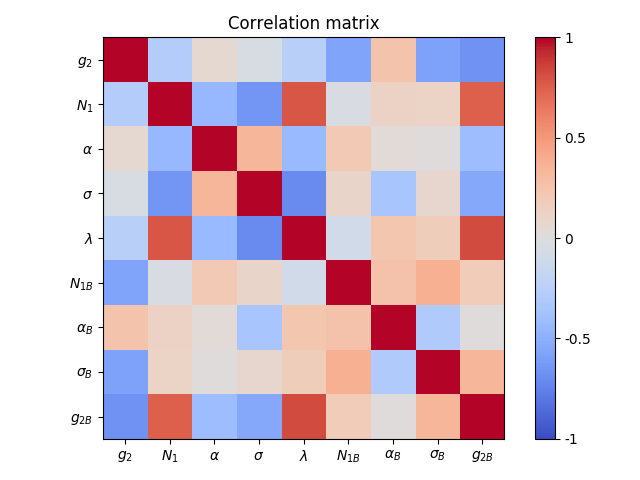
\includegraphics{pngplots/CorrelationMatrix.png}
\caption{Fitted parameter correlation matrix}
\end{figure}

\hypertarget{fit-properties}{%
\subsection{Fit properties}\label{fit-properties}}

\begin{figure}
\centering
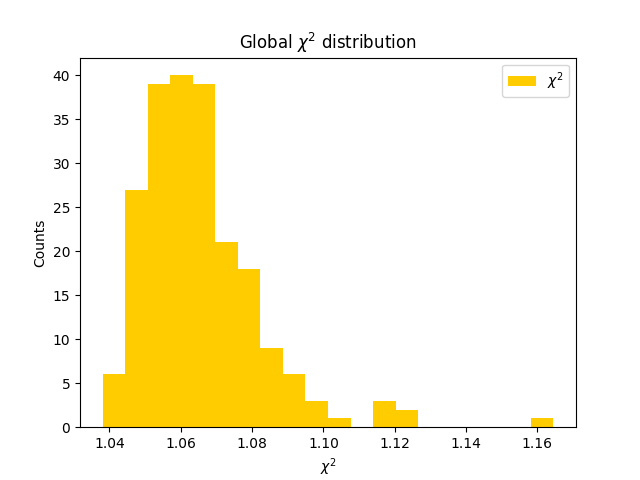
\includegraphics{pngplots/Globalchi2.png}
\caption{Global \(\chi^2\) distribution}
\end{figure}

\begin{figure}
\centering
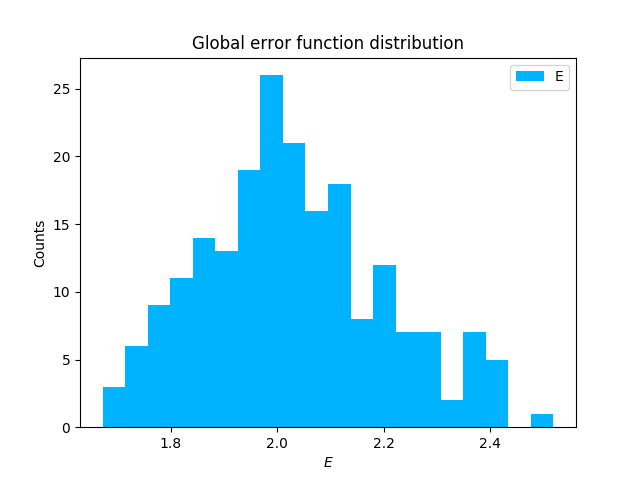
\includegraphics{pngplots/GlobalErrorFunction.png}
\caption{Global error function distribution}
\end{figure}

\begin{figure}
\centering
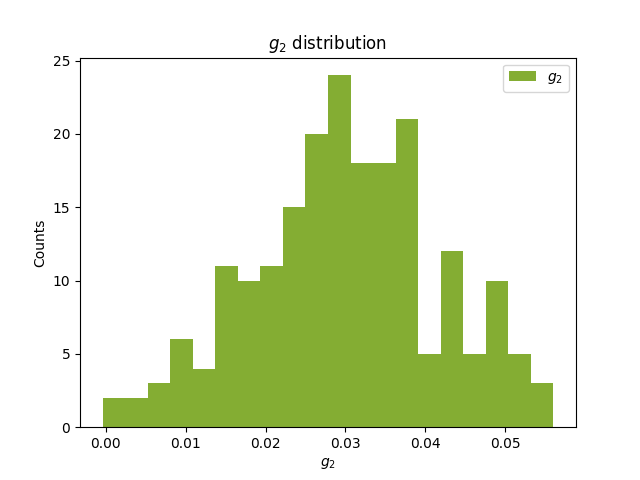
\includegraphics{pngplots/param0.png}
\caption{\(g_2\) distribution}
\end{figure}

\begin{figure}
\centering
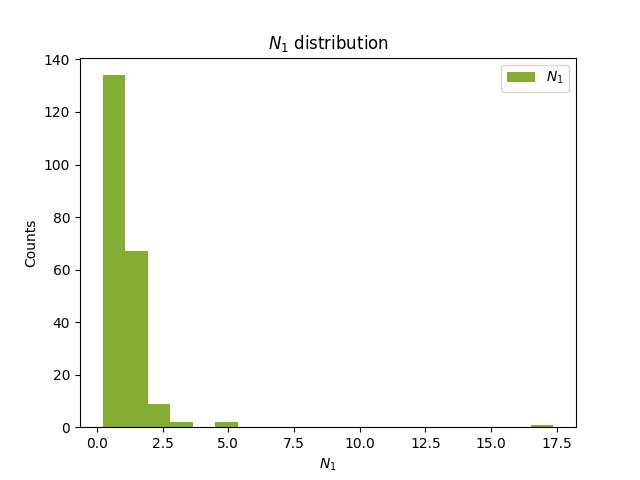
\includegraphics{pngplots/param1.png}
\caption{\(N_1\) distribution}
\end{figure}

\begin{figure}
\centering
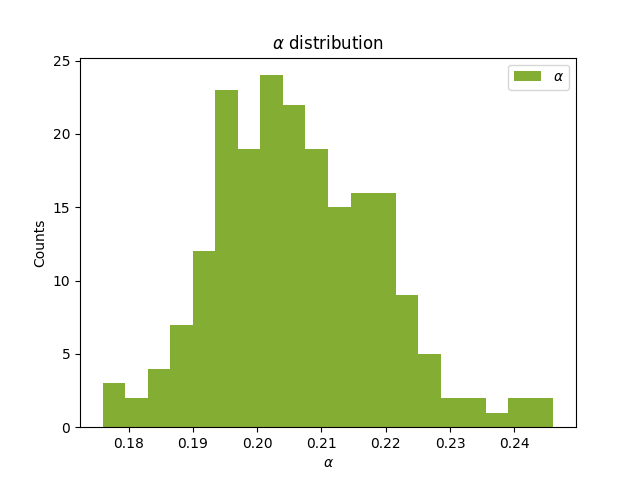
\includegraphics{pngplots/param2.png}
\caption{\(\alpha\) distribution}
\end{figure}

\begin{figure}
\centering
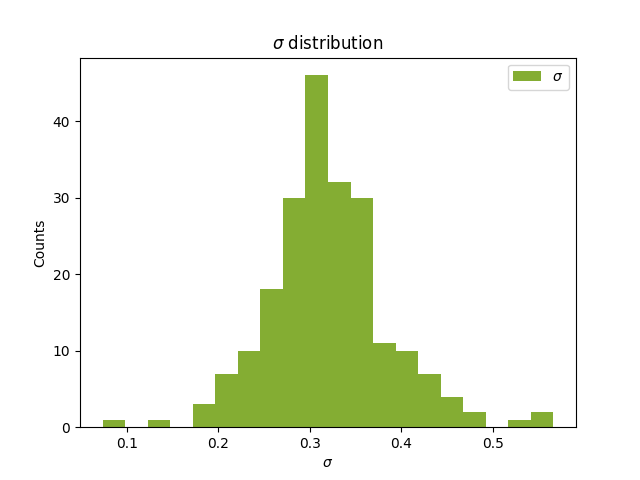
\includegraphics{pngplots/param3.png}
\caption{\(\sigma\) distribution}
\end{figure}

\begin{figure}
\centering
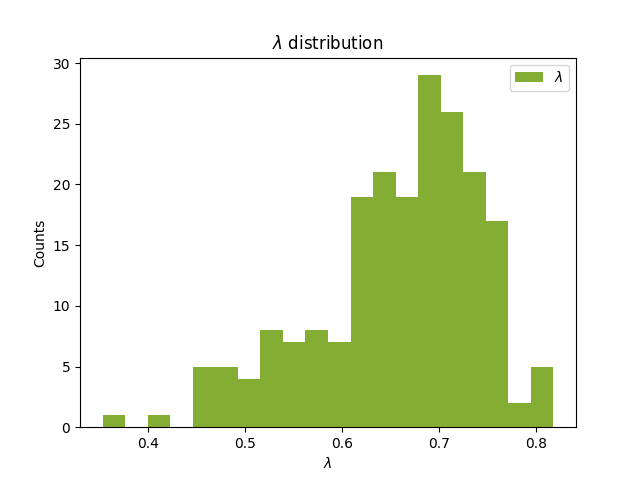
\includegraphics{pngplots/param4.png}
\caption{\(\lambda\) distribution}
\end{figure}

\begin{figure}
\centering
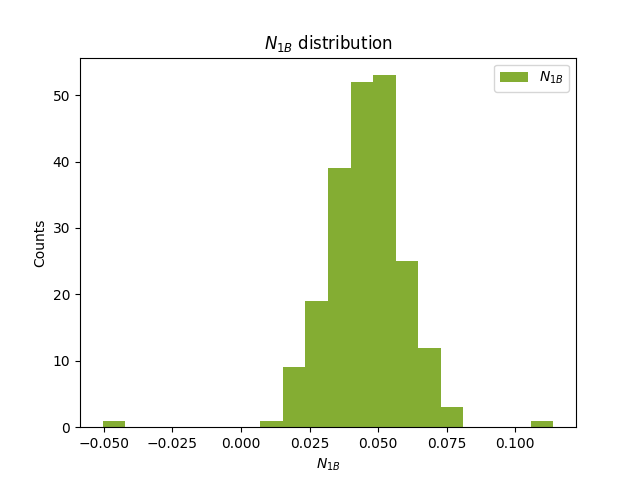
\includegraphics{pngplots/param5.png}
\caption{\(N_{1B}\) distribution}
\end{figure}

\begin{figure}
\centering
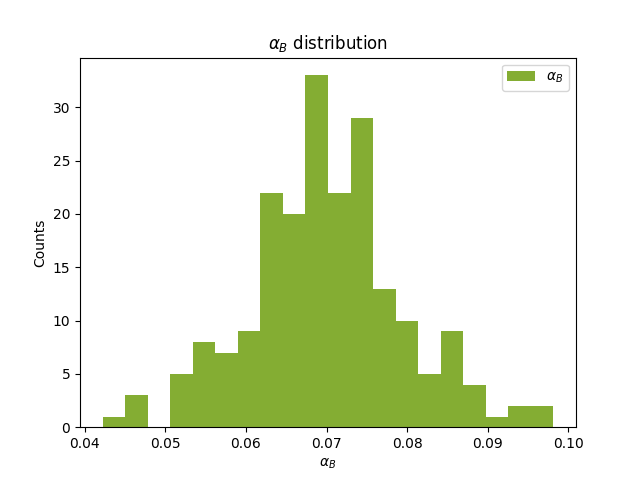
\includegraphics{pngplots/param6.png}
\caption{\(\alpha_B\) distribution}
\end{figure}

\begin{figure}
\centering
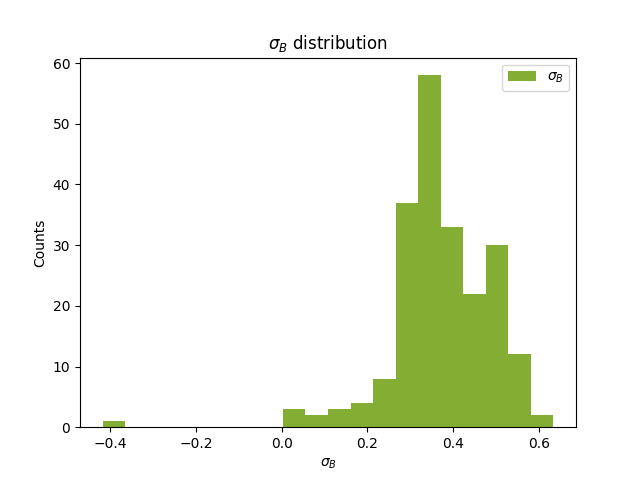
\includegraphics{pngplots/param7.png}
\caption{\(\sigma_B\) distribution}
\end{figure}

\begin{figure}
\centering
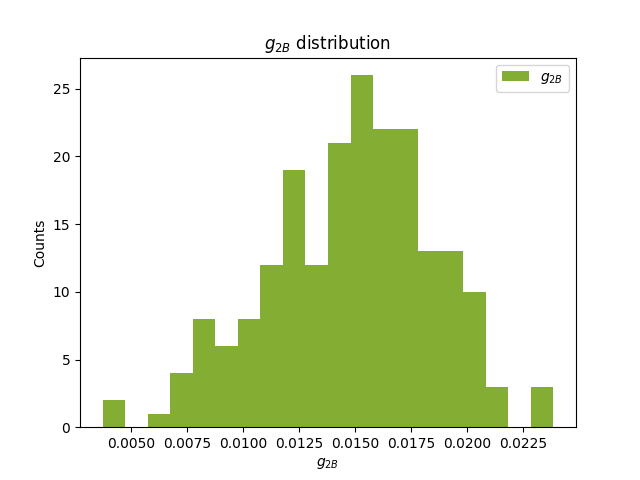
\includegraphics{pngplots/param8.png}
\caption{\(g_{2B}\) distribution}
\end{figure}

\hypertarget{table-of-chi2s}{%
\subsection{\texorpdfstring{Table of
\(\chi^2\)'s}{Table of \textbackslash chi\^{}2's}}\label{table-of-chi2s}}

\begin{table}[h]

\centering

\begin{tabular}{|c|c|c|c|c|} \hline

\textbf{Experiment} & \textbf{Number of
points} & \textbf{\(\chi_{D}^2\)} & \textbf{\(\chi_{\lambda}^2\)} & \textbf{\(\chi^2\)} \\ \hline

E605\_Q\_7\_8 & 7 & 0.6409 & 0.0014 & 0.6423 \\ \hline
E605\_Q\_8\_9 & 8 & 1.5475 & 0.0004 & 1.5479 \\ \hline
E605\_Q\_10.5\_11.5 & 10 & 0.4648 & 0.1565 & 0.6213 \\ \hline
E288\_200\_Q\_4\_5 & 4 & 0.6701 & 0.7756 & 1.4457 \\ \hline
E288\_200\_Q\_5\_6 & 5 & 1.6172 & 0.2007 & 1.8179 \\ \hline
E288\_200\_Q\_6\_7 & 6 & 0.367 & 0.1015 & 0.4684 \\ \hline
E288\_200\_Q\_7\_8 & 7 & 0.538 & 0.002 & 0.54 \\ \hline
E288\_200\_Q\_8\_9 & 8 & 0.5951 & 0.0477 & 0.6428 \\ \hline
E288\_300\_Q\_4\_5 & 4 & 0.5335 & 0.4563 & 0.9899 \\ \hline
E288\_300\_Q\_5\_6 & 5 & 0.838 & 0.1068 & 0.9448 \\ \hline
E288\_300\_Q\_6\_7 & 6 & 0.507 & 0.0182 & 0.5252 \\ \hline
E288\_300\_Q\_7\_8 & 7 & 0.1288 & 0.0069 & 0.1357 \\ \hline
E288\_300\_Q\_8\_9 & 8 & 0.4834 & 0.0016 & 0.485 \\ \hline
E288\_400\_Q\_5\_6 & 5 & 0.2955 & 0.0002 & 0.2958 \\ \hline
E288\_400\_Q\_6\_7 & 6 & 0.086 & 0.0052 & 0.0912 \\ \hline
E288\_400\_Q\_7\_8 & 7 & 0.0242 & 0.0291 & 0.0532 \\ \hline
E288\_400\_Q\_8\_9 & 8 & 0.4447 & 0.0557 & 0.5004 \\ \hline
E288\_400\_Q\_11\_12 & 11 & 0.5017 & 0.0636 & 0.5653 \\ \hline
E288\_400\_Q\_12\_13 & 12 & 0.4894 & 0.0552 & 0.5446 \\ \hline
E288\_400\_Q\_13\_14 & 12 & 0.6029 & 0.0978 & 0.7007 \\ \hline
STAR\_510 & 7 & 0.8882 & 0.0375 & 0.9257 \\ \hline
CDF\_RunI & 25 & 0.5319 & 0.0577 & 0.5896 \\ \hline
CDF\_RunII & 26 & 0.8466 & 0.0027 & 0.8493 \\ \hline
D0\_RunI & 12 & 0.597 & 0.0439 & 0.6409 \\ \hline
D0\_RunII & 5 & 0.9087 & 0.5825 & 1.4912 \\ \hline
D0\_RunIImu & 3 & 2.9385 & 0.0256 & 2.9641 \\ \hline
LHCb\_7TeV & 7 & 1.0896 & 0.1472 & 1.2368 \\ \hline
LHCb\_8TeV & 7 & 0.6181 & 0.1 & 0.7181 \\ \hline
LHCb\_13TeV & 7 & 0.8796 & 0.0262 & 0.9058 \\ \hline
CMS\_7TeV & 4 & 2.117 & 0 & 2.117 \\ \hline
CMS\_8TeV & 4 & 1.4011 & 0.0071 & 1.4082 \\ \hline
ATLAS\_7TeV\_y\_0\_1 & 6 & 2.5001 & 0.0276 & 2.5277 \\ \hline
ATLAS\_7TeV\_y\_1\_2 & 6 & 4.1178 & 1.0352 & 5.1529 \\ \hline
ATLAS\_7TeV\_y\_2\_2.4 & 6 & 3.5149 & 0.3817 & 3.8966 \\ \hline
ATLAS\_8TeV\_y\_0\_0.4 & 6 & 1.9202 & 0.3487 & 2.2689 \\ \hline
ATLAS\_8TeV\_y\_0.4\_0.8 & 6 & 2.1954 & 0.2606 & 2.4559 \\ \hline
ATLAS\_8TeV\_y\_0.8\_1.2 & 6 & 0.8627 & 0.0634 & 0.9261 \\ \hline
ATLAS\_8TeV\_y\_1.2\_1.6 & 6 & 0.8989 & 0.104 & 1.0028 \\ \hline
ATLAS\_8TeV\_y\_1.6\_2 & 6 & 0.5636 & 0.0738 & 0.6374 \\ \hline
ATLAS\_8TeV\_y\_2\_2.4 & 6 & 0.6445 & 0.279 & 0.9235 \\ \hline
ATLAS\_8TeV\_Q\_46\_66 & 4 & 2.2661 & 0.7195 & 2.9856 \\ \hline
ATLAS\_8TeV\_Q\_116\_150 & 8 & 0.4965 & 0.0032 & 0.4997 \\ \hline
Total & 319 & - & - & 1.0347 \\ \hline

\end{tabular}

\caption{Central-replica \(\chi^2\)'s:}

\end{table}

\begin{table}[h]

\centering

\begin{tabular}{|c|c|c|c|c|} \hline

\textbf{Experiment} & \textbf{Number of
points} & \textbf{\(\chi_{D}^2\)} & \textbf{\(\chi_{\lambda}^2\)} & \textbf{\(\chi^2\)} \\ \hline

E605\_Q\_7\_8 & 7 & 0.5534 & 0.027 & 0.5804 \\ \hline
E605\_Q\_8\_9 & 8 & 1.1713 & 0.0285 & 1.1998 \\ \hline
E605\_Q\_10.5\_11.5 & 10 & 0.2253 & 0.1561 & 0.3815 \\ \hline
E288\_200\_Q\_4\_5 & 4 & 0.2585 & 0.4542 & 0.7127 \\ \hline
E288\_200\_Q\_5\_6 & 5 & 0.9114 & 0.2126 & 1.124 \\ \hline
E288\_200\_Q\_6\_7 & 6 & 0.2511 & 0.1147 & 0.3659 \\ \hline
E288\_200\_Q\_7\_8 & 7 & 0.5005 & 0.0132 & 0.5136 \\ \hline
E288\_200\_Q\_8\_9 & 8 & 0.7986 & 0.02 & 0.8186 \\ \hline
E288\_300\_Q\_4\_5 & 4 & 0.2503 & 0.3456 & 0.5959 \\ \hline
E288\_300\_Q\_5\_6 & 5 & 0.5547 & 0.152 & 0.7067 \\ \hline
E288\_300\_Q\_6\_7 & 6 & 0.4545 & 0.0487 & 0.5032 \\ \hline
E288\_300\_Q\_7\_8 & 7 & 0.1387 & 0.0215 & 0.1602 \\ \hline
E288\_300\_Q\_8\_9 & 8 & 0.3972 & 0.0109 & 0.408 \\ \hline
E288\_400\_Q\_5\_6 & 5 & 0.2878 & 0.0253 & 0.3131 \\ \hline
E288\_400\_Q\_6\_7 & 6 & 0.1049 & 0.0022 & 0.1071 \\ \hline
E288\_400\_Q\_7\_8 & 7 & 0.0375 & 0.01 & 0.0475 \\ \hline
E288\_400\_Q\_8\_9 & 8 & 0.5503 & 0.0432 & 0.5935 \\ \hline
E288\_400\_Q\_11\_12 & 11 & 0.6806 & 0.0687 & 0.7493 \\ \hline
E288\_400\_Q\_12\_13 & 12 & 0.7923 & 0.0496 & 0.8419 \\ \hline
E288\_400\_Q\_13\_14 & 12 & 1.1274 & 0.0596 & 1.187 \\ \hline
STAR\_510 & 7 & 0.7653 & 0.0612 & 0.8265 \\ \hline
CDF\_RunI & 25 & 0.4703 & 0.0594 & 0.5296 \\ \hline
CDF\_RunII & 26 & 0.8568 & 0.0007 & 0.8575 \\ \hline
D0\_RunI & 12 & 0.65 & 0.0402 & 0.6902 \\ \hline
D0\_RunII & 5 & 0.8905 & 0.5827 & 1.4732 \\ \hline
D0\_RunIImu & 3 & 2.9186 & 0.0261 & 2.9447 \\ \hline
LHCb\_7TeV & 7 & 1.0259 & 0.1649 & 1.1908 \\ \hline
LHCb\_8TeV & 7 & 0.6459 & 0.0956 & 0.7415 \\ \hline
LHCb\_13TeV & 7 & 0.8563 & 0.0249 & 0.8812 \\ \hline
CMS\_7TeV & 4 & 2.1183 & 0 & 2.1183 \\ \hline
CMS\_8TeV & 4 & 1.4613 & 0.0051 & 1.4664 \\ \hline
ATLAS\_7TeV\_y\_0\_1 & 6 & 3.0761 & 0.0351 & 3.1112 \\ \hline
ATLAS\_7TeV\_y\_1\_2 & 6 & 4.2003 & 1.082 & 5.2823 \\ \hline
ATLAS\_7TeV\_y\_2\_2.4 & 6 & 3.5882 & 0.3841 & 3.9722 \\ \hline
ATLAS\_8TeV\_y\_0\_0.4 & 6 & 1.9839 & 0.3606 & 2.3445 \\ \hline
ATLAS\_8TeV\_y\_0.4\_0.8 & 6 & 2.0855 & 0.3273 & 2.4128 \\ \hline
ATLAS\_8TeV\_y\_0.8\_1.2 & 6 & 1.0573 & 0.0911 & 1.1484 \\ \hline
ATLAS\_8TeV\_y\_1.2\_1.6 & 6 & 0.8265 & 0.096 & 0.9224 \\ \hline
ATLAS\_8TeV\_y\_1.6\_2 & 6 & 0.6823 & 0.0118 & 0.6941 \\ \hline
ATLAS\_8TeV\_y\_2\_2.4 & 6 & 0.5843 & 0.24 & 0.8244 \\ \hline
ATLAS\_8TeV\_Q\_46\_66 & 4 & 2.4774 & 0.6449 & 3.1223 \\ \hline
ATLAS\_8TeV\_Q\_116\_150 & 8 & 0.4942 & 0.0026 & 0.4968 \\ \hline
Total & 319 & - & - & 1.0409 \\ \hline

\end{tabular}

\caption{Mean-replica \(\chi^2\)'s:}

\end{table}

\begin{table}[h]

\centering

\begin{tabular}{|c|c|c|c|c|} \hline

\textbf{Experiment} & \textbf{Number of
points} & \textbf{\(\chi_{D}^2\)} & \textbf{\(\chi_{\lambda}^2\)} & \textbf{\(\chi^2\)} \\ \hline

E605\_Q\_7\_8 & 7 & 0.5301 \(\pm\) 0.2036 & 0.1336 \(\pm\)
0.1703 & 0.6637 \(\pm\) 0.1119 \\ \hline
E605\_Q\_8\_9 & 8 & 1.4211 \(\pm\) 0.2676 & 0.0968 \(\pm\)
0.1303 & 1.5179 \(\pm\) 0.2384 \\ \hline
E605\_Q\_10.5\_11.5 & 10 & 0.4292 \(\pm\) 0.3032 & 0.2265 \(\pm\)
0.2673 & 0.6557 \(\pm\) 0.1126 \\ \hline
E288\_200\_Q\_4\_5 & 4 & 0.2302 \(\pm\) 1.5175 & 1.2712 \(\pm\)
1.4492 & 1.5013 \(\pm\) 0.3342 \\ \hline
E288\_200\_Q\_5\_6 & 5 & 1.3792 \(\pm\) 0.7025 & 0.4833 \(\pm\)
0.6399 & 1.8625 \(\pm\) 0.2392 \\ \hline
E288\_200\_Q\_6\_7 & 6 & 0.1591 \(\pm\) 0.4359 & 0.3401 \(\pm\)
0.4263 & 0.4991 \(\pm\) 0.1105 \\ \hline
E288\_200\_Q\_7\_8 & 7 & 0.3682 \(\pm\) 0.2832 & 0.1817 \(\pm\)
0.2315 & 0.55 \(\pm\) 0.1695 \\ \hline
E288\_200\_Q\_8\_9 & 8 & 0.5094 \(\pm\) 0.1565 & 0.1375 \(\pm\)
0.1524 & 0.647 \(\pm\) 0.0852 \\ \hline
E288\_300\_Q\_4\_5 & 4 & 0.2107 \(\pm\) 1.1718 & 0.8513 \(\pm\)
1.0855 & 1.0619 \(\pm\) 0.2725 \\ \hline
E288\_300\_Q\_5\_6 & 5 & 0.6533 \(\pm\) 0.5022 & 0.3446 \(\pm\)
0.4636 & 0.9978 \(\pm\) 0.1492 \\ \hline
E288\_300\_Q\_6\_7 & 6 & 0.3655 \(\pm\) 0.2934 & 0.1811 \(\pm\)
0.2521 & 0.5466 \(\pm\) 0.1418 \\ \hline
E288\_300\_Q\_7\_8 & 7 & -0.0046 \(\pm\) 0.2119 & 0.154 \(\pm\)
0.1983 & 0.1494 \(\pm\) 0.058 \\ \hline
E288\_300\_Q\_8\_9 & 8 & 0.404 \(\pm\) 0.1581 & 0.1061 \(\pm\)
0.1451 & 0.5101 \(\pm\) 0.0894 \\ \hline
E288\_400\_Q\_5\_6 & 5 & 0.1473 \(\pm\) 0.3078 & 0.2129 \(\pm\)
0.2788 & 0.3603 \(\pm\) 0.1138 \\ \hline
E288\_400\_Q\_6\_7 & 6 & -0.0051 \(\pm\) 0.1924 & 0.1356 \(\pm\)
0.1884 & 0.1306 \(\pm\) 0.0523 \\ \hline
E288\_400\_Q\_7\_8 & 7 & -0.0436 \(\pm\) 0.1961 & 0.1402 \(\pm\)
0.1833 & 0.0966 \(\pm\) 0.077 \\ \hline
E288\_400\_Q\_8\_9 & 8 & 0.3883 \(\pm\) 0.2187 & 0.156 \(\pm\)
0.2056 & 0.5443 \(\pm\) 0.113 \\ \hline
E288\_400\_Q\_11\_12 & 11 & 0.4861 \(\pm\) 0.2055 & 0.121 \(\pm\)
0.1339 & 0.6071 \(\pm\) 0.1649 \\ \hline
E288\_400\_Q\_12\_13 & 12 & 0.4542 \(\pm\) 0.1483 & 0.1256 \(\pm\)
0.1411 & 0.5798 \(\pm\) 0.0504 \\ \hline
E288\_400\_Q\_13\_14 & 12 & 0.5777 \(\pm\) 0.1357 & 0.1356 \(\pm\)
0.123 & 0.7133 \(\pm\) 0.0572 \\ \hline
STAR\_510 & 7 & 0.8069 \(\pm\) 0.2044 & 0.1415 \(\pm\) 0.2011 & 0.9484
\(\pm\) 0.0579 \\ \hline
CDF\_RunI & 25 & 0.4989 \(\pm\) 0.1137 & 0.0971 \(\pm\) 0.1124 & 0.5959
\(\pm\) 0.0177 \\ \hline
CDF\_RunII & 26 & 0.8392 \(\pm\) 0.0807 & 0.043 \(\pm\) 0.051 & 0.8822
\(\pm\) 0.0613 \\ \hline
D0\_RunI & 12 & 0.544 \(\pm\) 0.1419 & 0.103 \(\pm\) 0.1362 & 0.647
\(\pm\) 0.037 \\ \hline
D0\_RunII & 5 & 0.7611 \(\pm\) 0.7485 & 0.7627 \(\pm\) 0.7308 & 1.5237
\(\pm\) 0.2302 \\ \hline
D0\_RunIImu & 3 & 2.4048 \(\pm\) 0.8891 & 0.5369 \(\pm\) 0.5761 & 2.9417
\(\pm\) 0.6618 \\ \hline
LHCb\_7TeV & 7 & 0.8998 \(\pm\) 0.3477 & 0.3593 \(\pm\) 0.3473 & 1.2591
\(\pm\) 0.0511 \\ \hline
LHCb\_8TeV & 7 & 0.5211 \(\pm\) 0.3402 & 0.2406 \(\pm\) 0.2962 & 0.7617
\(\pm\) 0.1913 \\ \hline
LHCb\_13TeV & 7 & 0.8459 \(\pm\) 0.1969 & 0.107 \(\pm\) 0.151 & 0.9529
\(\pm\) 0.1333 \\ \hline
CMS\_7TeV & 4 & 2.1221 \(\pm\) 0.012 & 0.0 \(\pm\) 0.0 & 2.1221 \(\pm\)
0.012 \\ \hline
CMS\_8TeV & 4 & 1.341 \(\pm\) 0.1187 & 0.0683 \(\pm\) 0.1018 & 1.4092
\(\pm\) 0.058 \\ \hline
ATLAS\_7TeV\_y\_0\_1 & 6 & 2.5017 \(\pm\) 0.312 & 0.0999 \(\pm\)
0.1481 & 2.6016 \(\pm\) 0.2743 \\ \hline
ATLAS\_7TeV\_y\_1\_2 & 6 & 4.2127 \(\pm\) 0.4745 & 1.0264 \(\pm\)
0.4413 & 5.2391 \(\pm\) 0.1288 \\ \hline
ATLAS\_7TeV\_y\_2\_2.4 & 6 & 3.5284 \(\pm\) 0.2071 & 0.4086 \(\pm\)
0.1603 & 3.937 \(\pm\) 0.1314 \\ \hline
ATLAS\_8TeV\_y\_0\_0.4 & 6 & 1.9146 \(\pm\) 0.3393 & 0.3852 \(\pm\)
0.2909 & 2.2998 \(\pm\) 0.1527 \\ \hline
ATLAS\_8TeV\_y\_0.4\_0.8 & 6 & 2.1413 \(\pm\) 0.329 & 0.3546 \(\pm\)
0.3138 & 2.4958 \(\pm\) 0.1229 \\ \hline
ATLAS\_8TeV\_y\_0.8\_1.2 & 6 & 0.8871 \(\pm\) 0.1651 & 0.1014 \(\pm\)
0.1209 & 0.9886 \(\pm\) 0.0991 \\ \hline
ATLAS\_8TeV\_y\_1.2\_1.6 & 6 & 0.8677 \(\pm\) 0.2508 & 0.1659 \(\pm\)
0.1836 & 1.0337 \(\pm\) 0.1676 \\ \hline
ATLAS\_8TeV\_y\_1.6\_2 & 6 & 0.6278 \(\pm\) 0.3359 & 0.1395 \(\pm\)
0.1784 & 0.7673 \(\pm\) 0.2658 \\ \hline
ATLAS\_8TeV\_y\_2\_2.4 & 6 & 0.6623 \(\pm\) 0.4017 & 0.3339 \(\pm\)
0.2603 & 0.9962 \(\pm\) 0.2806 \\ \hline
ATLAS\_8TeV\_Q\_46\_66 & 4 & 2.1045 \(\pm\) 0.6727 & 0.8761 \(\pm\)
0.658 & 2.9806 \(\pm\) 0.1231 \\ \hline
ATLAS\_8TeV\_Q\_116\_150 & 8 & 0.4079 \(\pm\) 0.1662 & 0.0979 \(\pm\)
0.165 & 0.5058 \(\pm\) 0.0114 \\ \hline
Total & 319 & - & - & 1.0655 \(\pm\) 0.0169 \\ \hline

\end{tabular}

\caption{Average-over-replicas \(\chi^2\)'s:}

\end{table}

\hypertarget{tmds-in-k_t-space}{%
\subsection{\texorpdfstring{TMDs in \(k_T\)
space}{TMDs in k\_T space}}\label{tmds-in-k_t-space}}

\begin{figure}
\centering
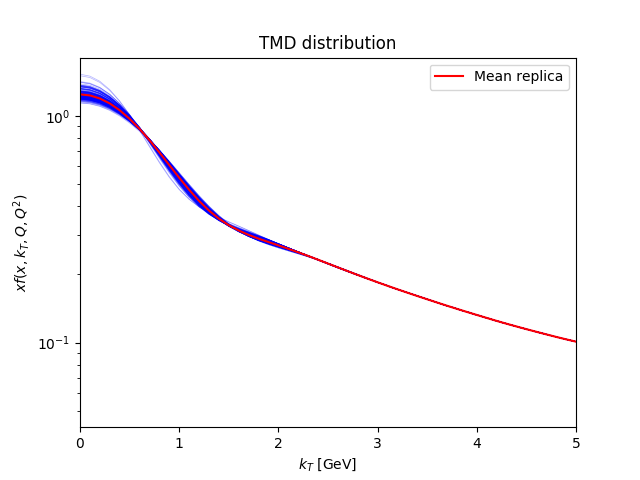
\includegraphics{pngplots/tmd_1_2_0.001.png}
\caption{TMD PDF of the \(d\) at \(Q = 2\) GeV and \(x = 0.001\)}
\end{figure}

\begin{figure}
\centering
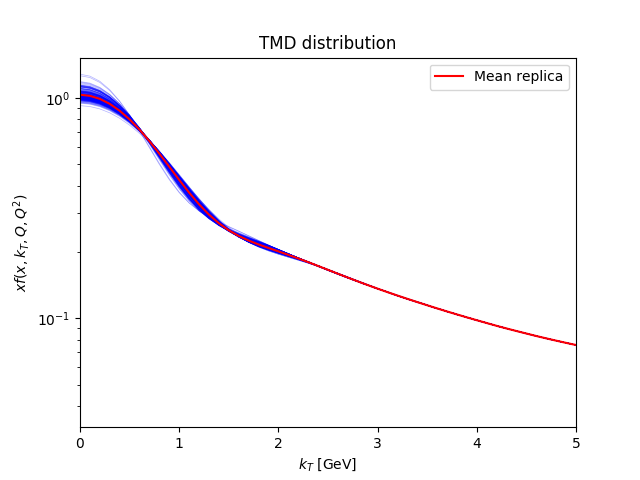
\includegraphics{pngplots/tmd_1_2_0.01.png}
\caption{TMD PDF of the \(d\) at \(Q = 2\) GeV and \(x = 0.01\)}
\end{figure}

\begin{figure}
\centering
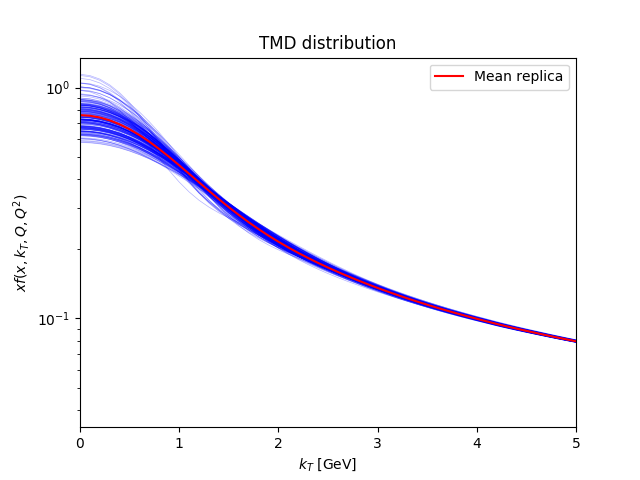
\includegraphics{pngplots/tmd_1_2_0.1.png}
\caption{TMD PDF of the \(d\) at \(Q = 2\) GeV and \(x = 0.1\)}
\end{figure}

\begin{figure}
\centering
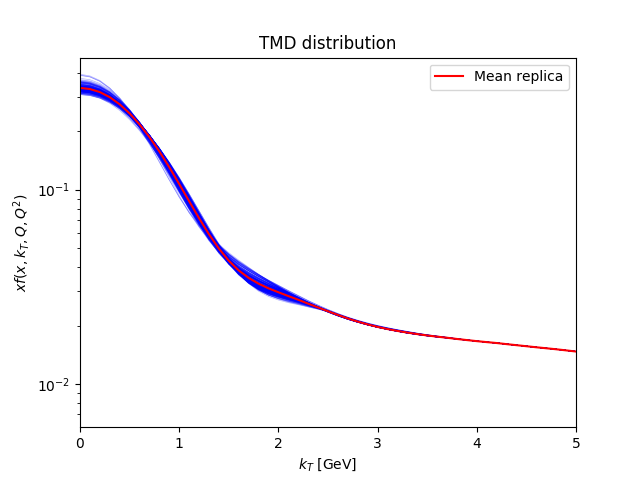
\includegraphics{pngplots/tmd_1_2_0.5.png}
\caption{TMD PDF of the \(d\) at \(Q = 2\) GeV and \(x = 0.5\)}
\end{figure}

\begin{figure}
\centering
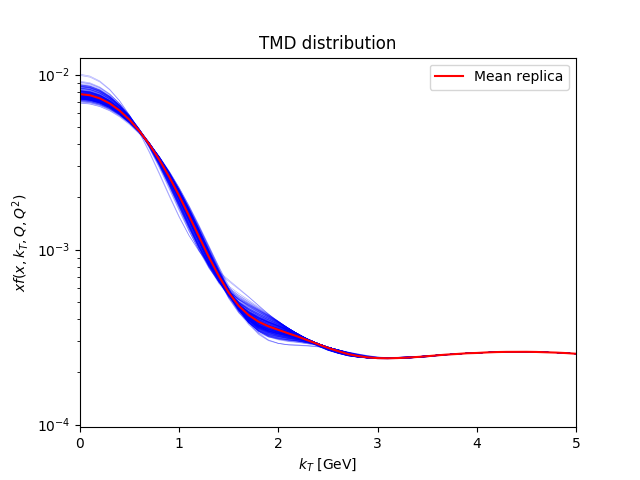
\includegraphics{pngplots/tmd_1_2_0.9.png}
\caption{TMD PDF of the \(d\) at \(Q = 2\) GeV and \(x = 0.9\)}
\end{figure}

\hypertarget{data-theory-comparison}{%
\subsection{Data-theory comparison}\label{data-theory-comparison}}

\begin{figure}
\centering
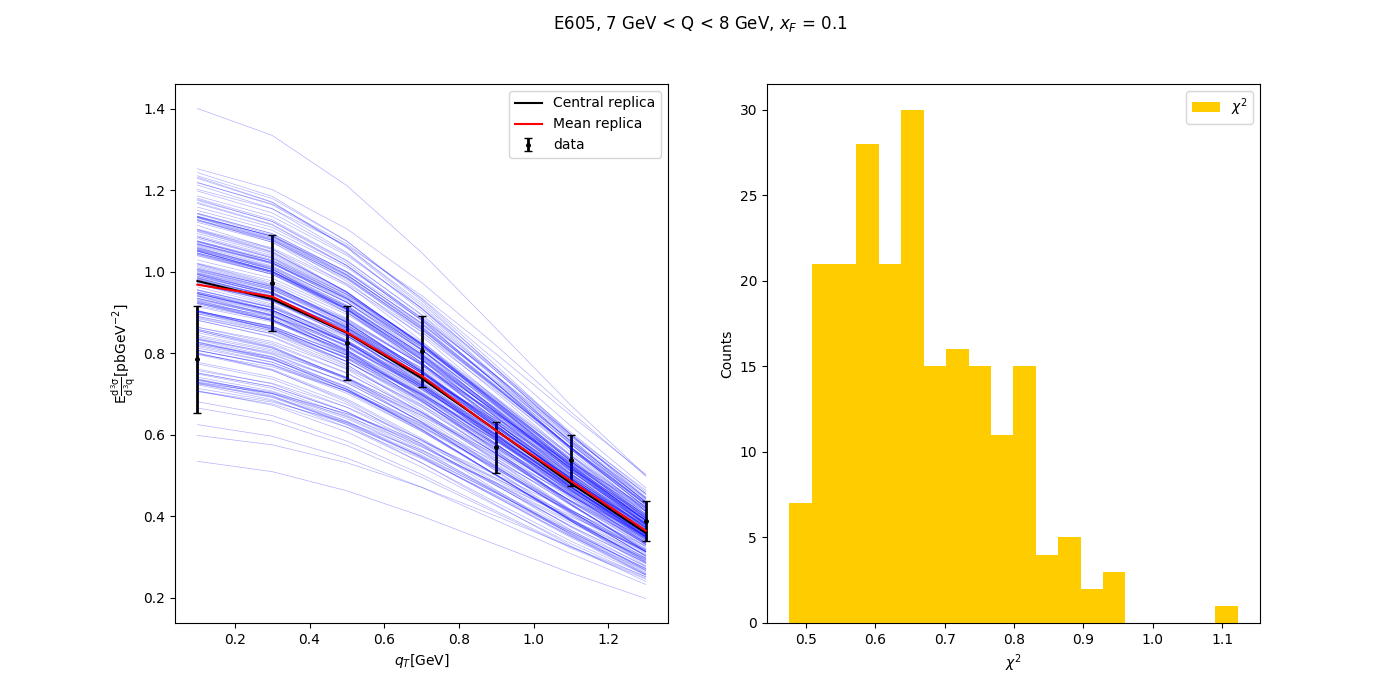
\includegraphics{pngplots/E605_Q_7_8.png}
\caption{E605\_Q\_7\_8 data-theory comparison}
\end{figure}

\begin{figure}
\centering
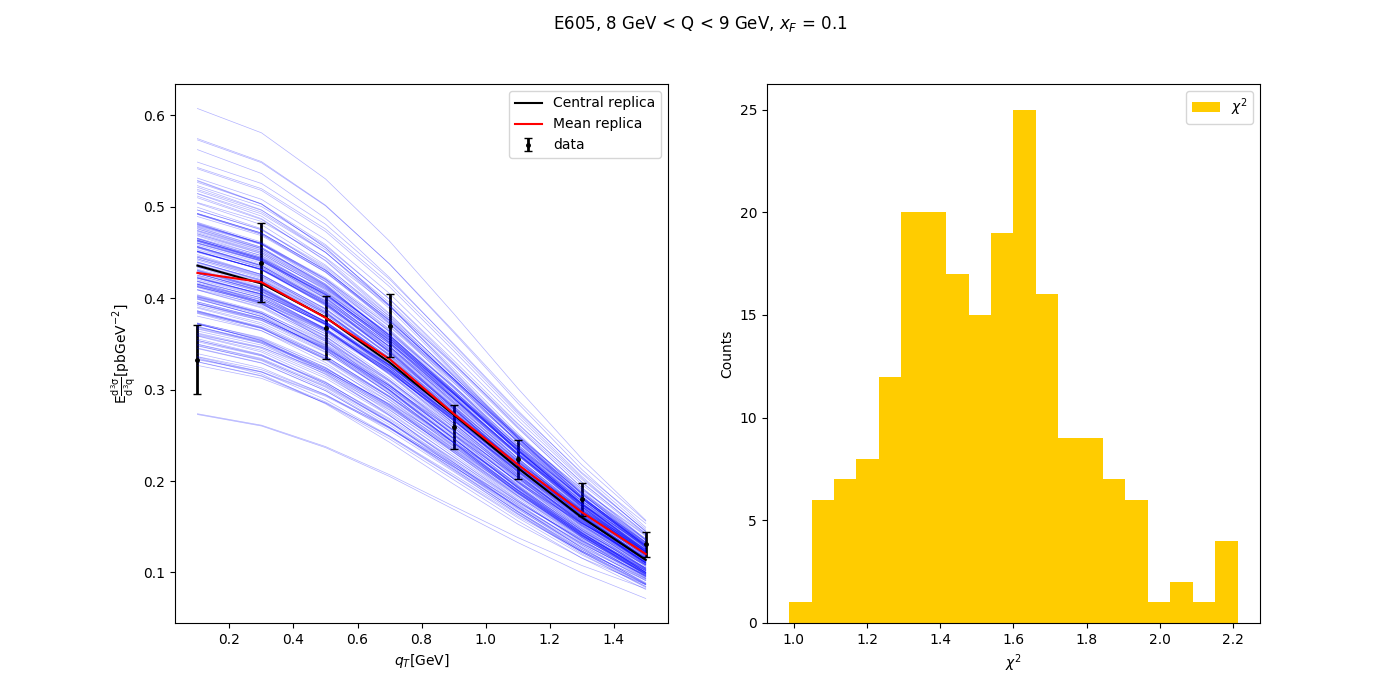
\includegraphics{pngplots/E605_Q_8_9.png}
\caption{E605\_Q\_8\_9 data-theory comparison}
\end{figure}

\begin{figure}
\centering
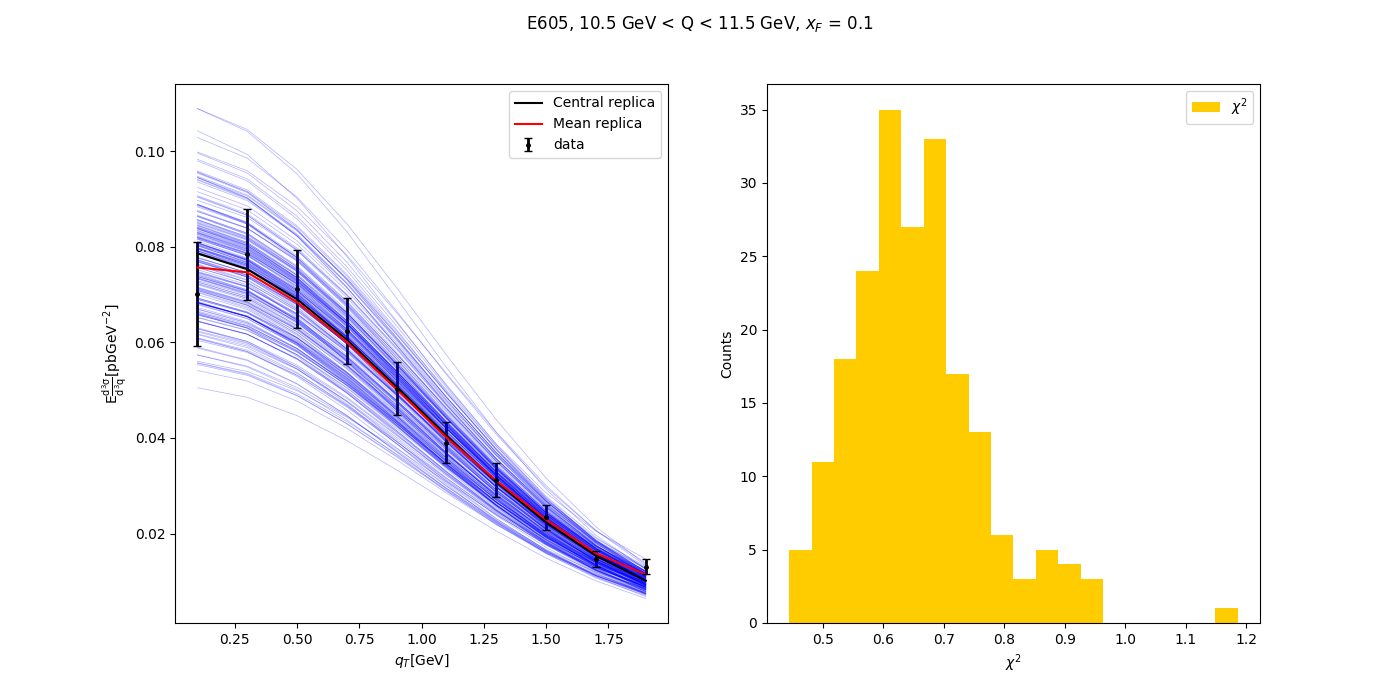
\includegraphics{pngplots/E605_Q_10.5_11.5.png}
\caption{E605\_Q\_10.5\_11.5 data-theory comparison}
\end{figure}

\begin{figure}
\centering
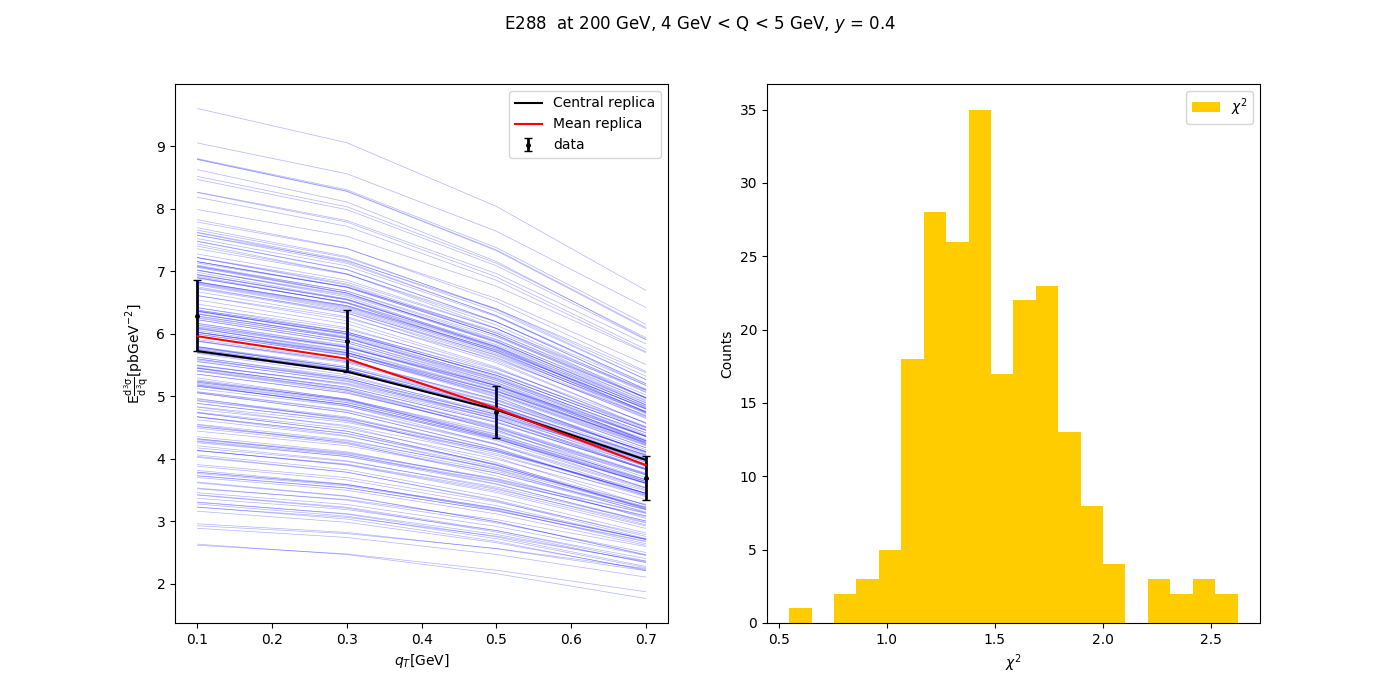
\includegraphics{pngplots/E288_200_Q_4_5.png}
\caption{E288\_200\_Q\_4\_5 data-theory comparison}
\end{figure}

\begin{figure}
\centering
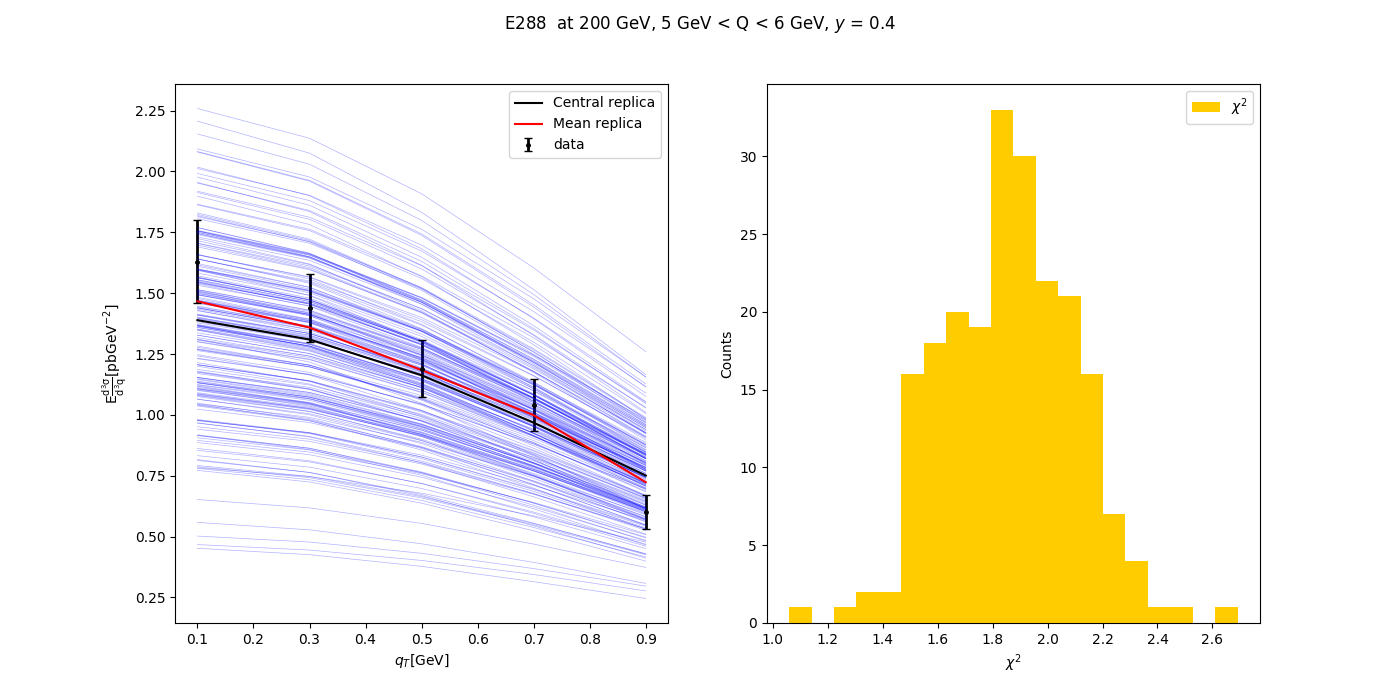
\includegraphics{pngplots/E288_200_Q_5_6.png}
\caption{E288\_200\_Q\_5\_6 data-theory comparison}
\end{figure}

\begin{figure}
\centering
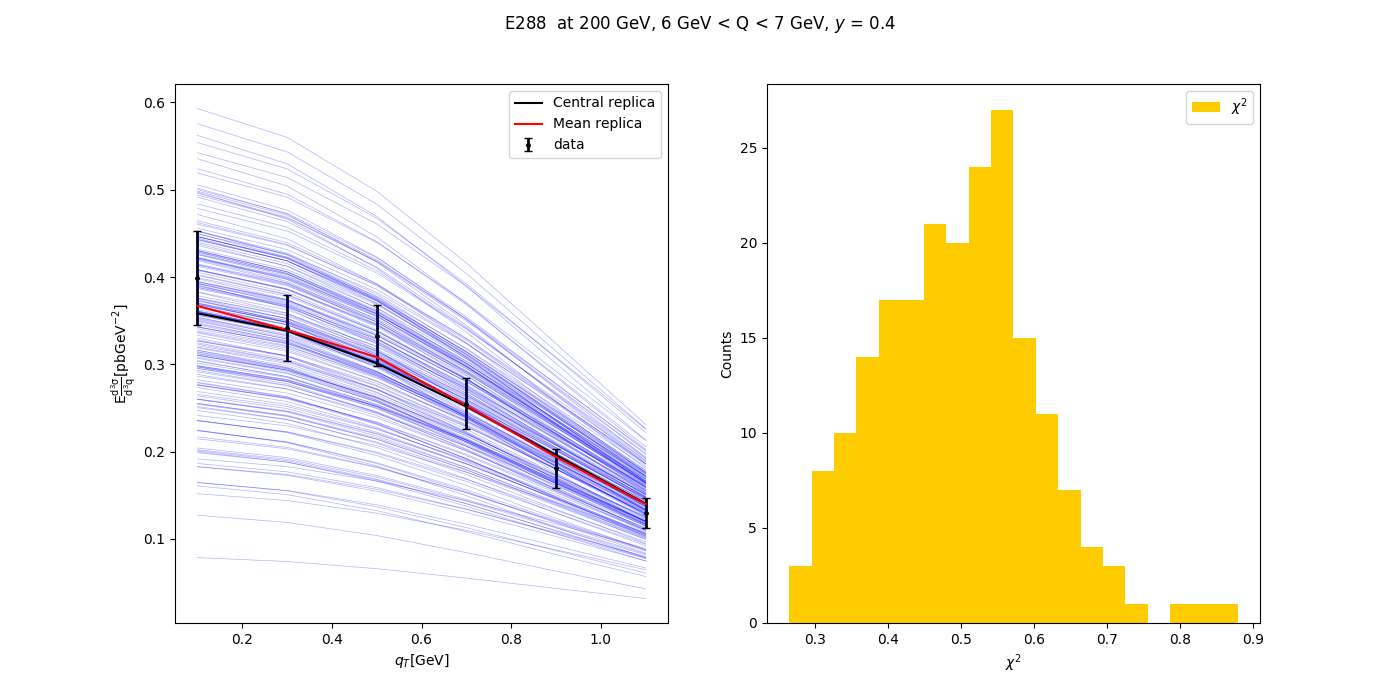
\includegraphics{pngplots/E288_200_Q_6_7.png}
\caption{E288\_200\_Q\_6\_7 data-theory comparison}
\end{figure}

\begin{figure}
\centering
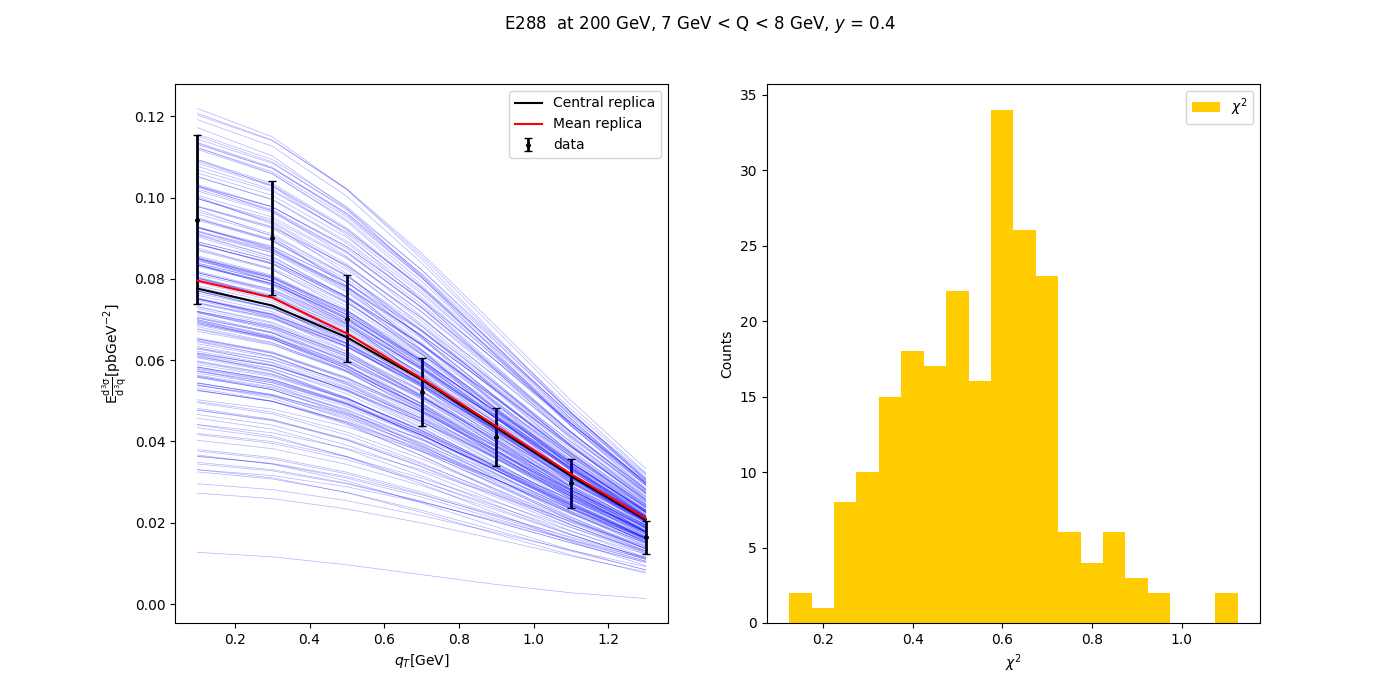
\includegraphics{pngplots/E288_200_Q_7_8.png}
\caption{E288\_200\_Q\_7\_8 data-theory comparison}
\end{figure}

\begin{figure}
\centering
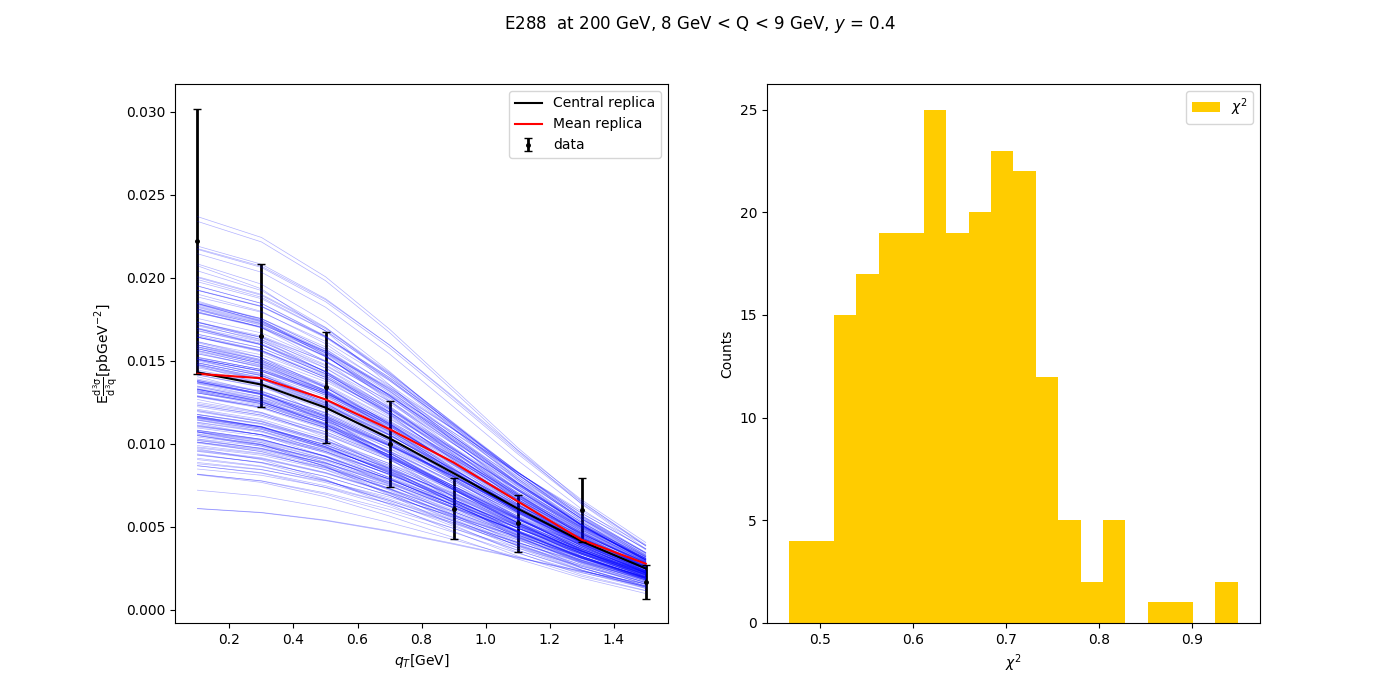
\includegraphics{pngplots/E288_200_Q_8_9.png}
\caption{E288\_200\_Q\_8\_9 data-theory comparison}
\end{figure}

\begin{figure}
\centering
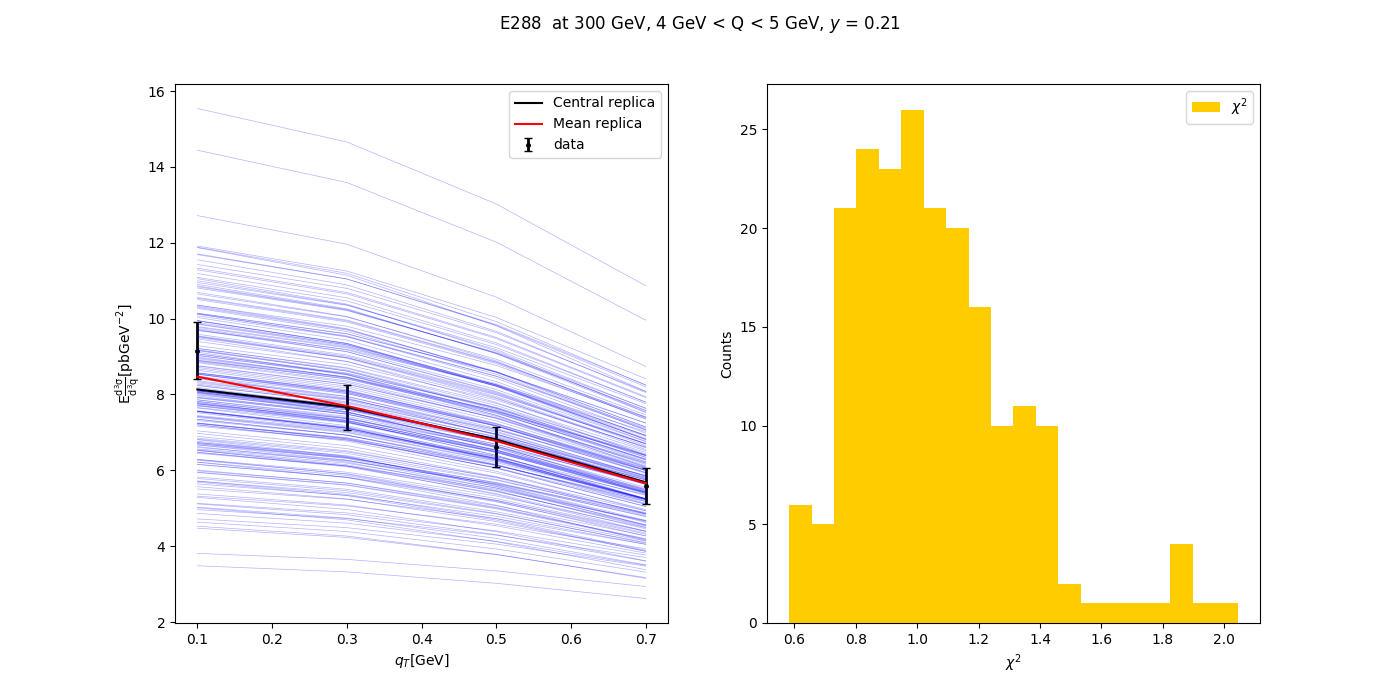
\includegraphics{pngplots/E288_300_Q_4_5.png}
\caption{E288\_300\_Q\_4\_5 data-theory comparison}
\end{figure}

\begin{figure}
\centering
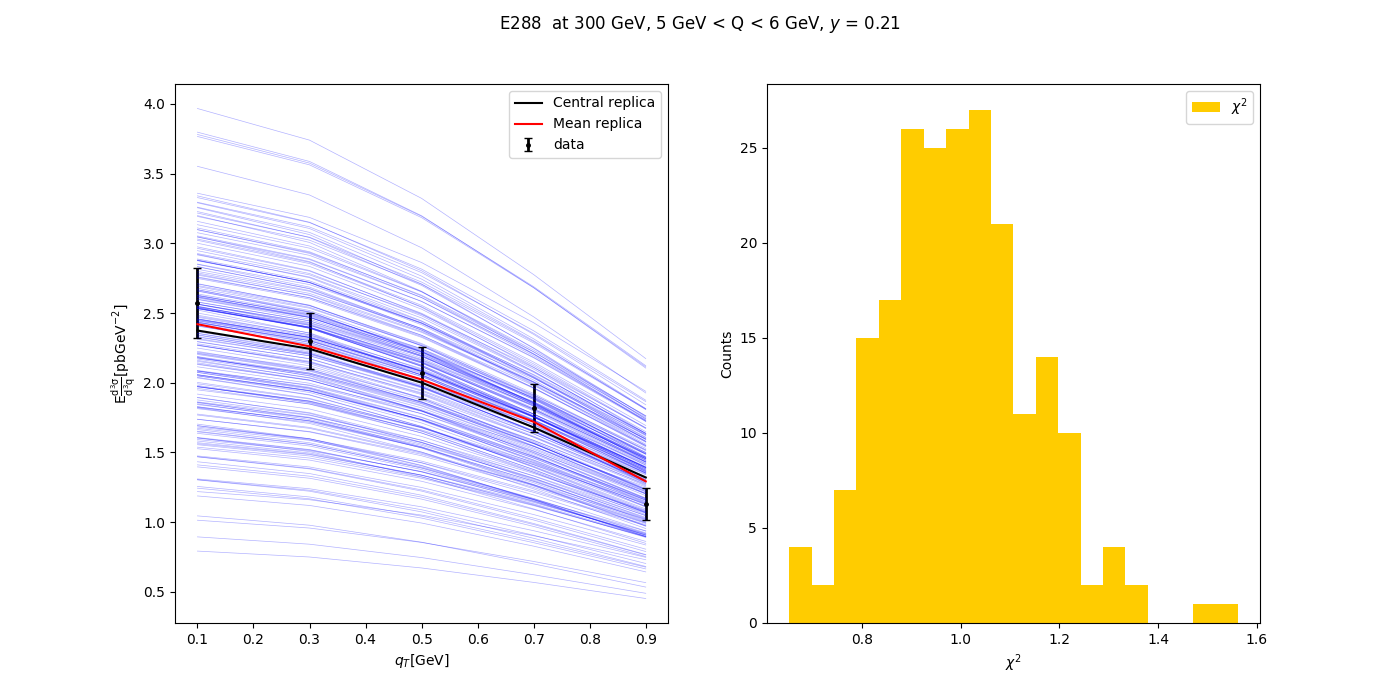
\includegraphics{pngplots/E288_300_Q_5_6.png}
\caption{E288\_300\_Q\_5\_6 data-theory comparison}
\end{figure}

\begin{figure}
\centering
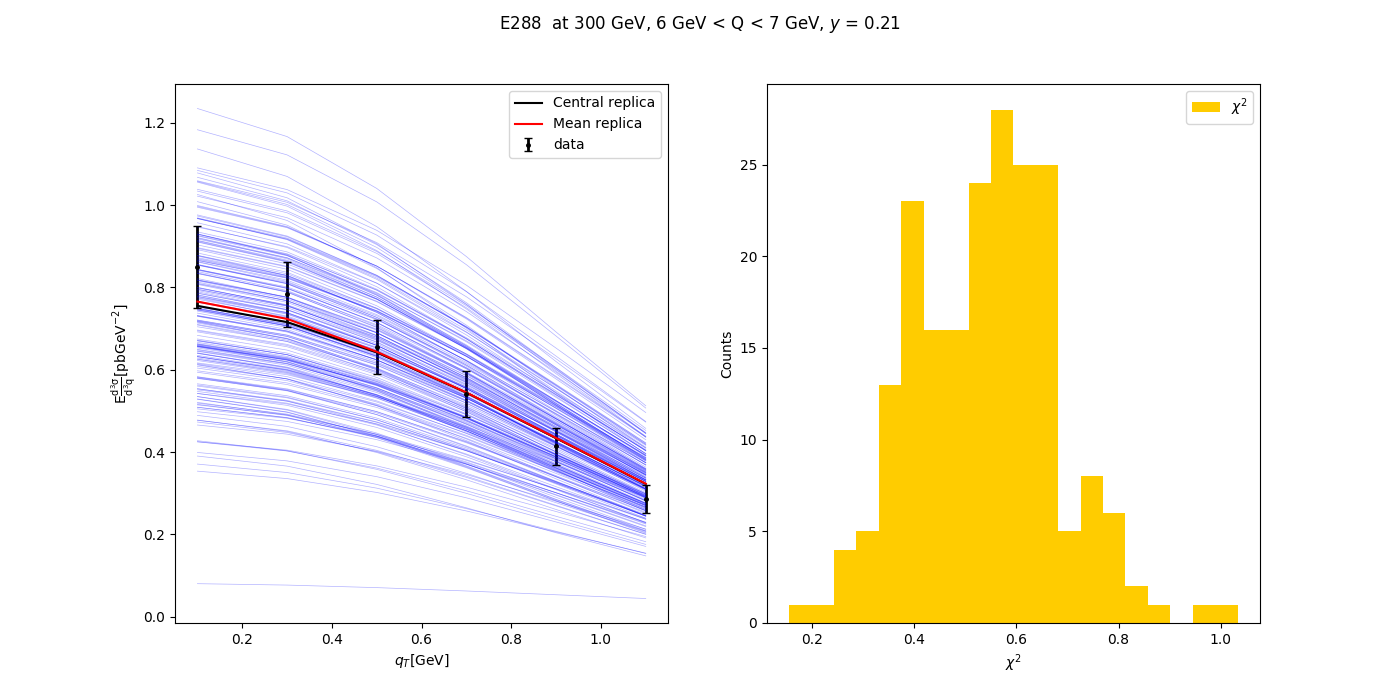
\includegraphics{pngplots/E288_300_Q_6_7.png}
\caption{E288\_300\_Q\_6\_7 data-theory comparison}
\end{figure}

\begin{figure}
\centering
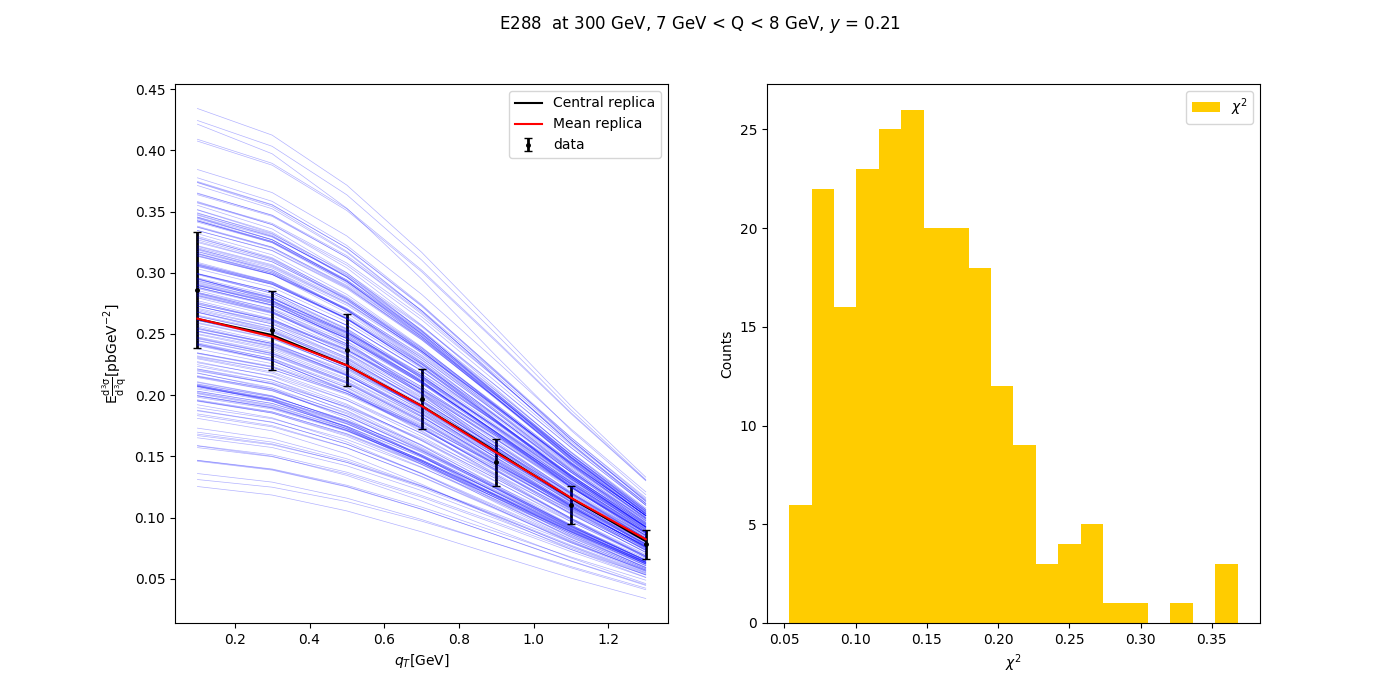
\includegraphics{pngplots/E288_300_Q_7_8.png}
\caption{E288\_300\_Q\_7\_8 data-theory comparison}
\end{figure}

\begin{figure}
\centering
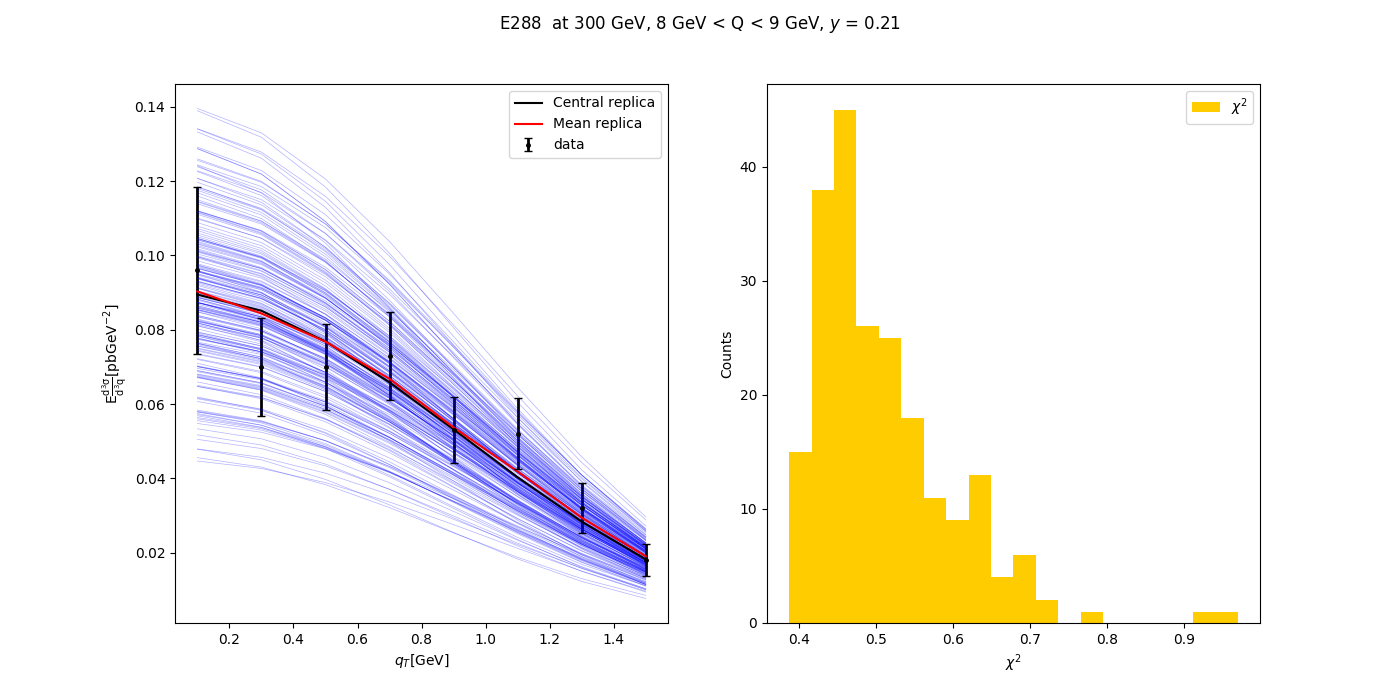
\includegraphics{pngplots/E288_300_Q_8_9.png}
\caption{E288\_300\_Q\_8\_9 data-theory comparison}
\end{figure}

\begin{figure}
\centering
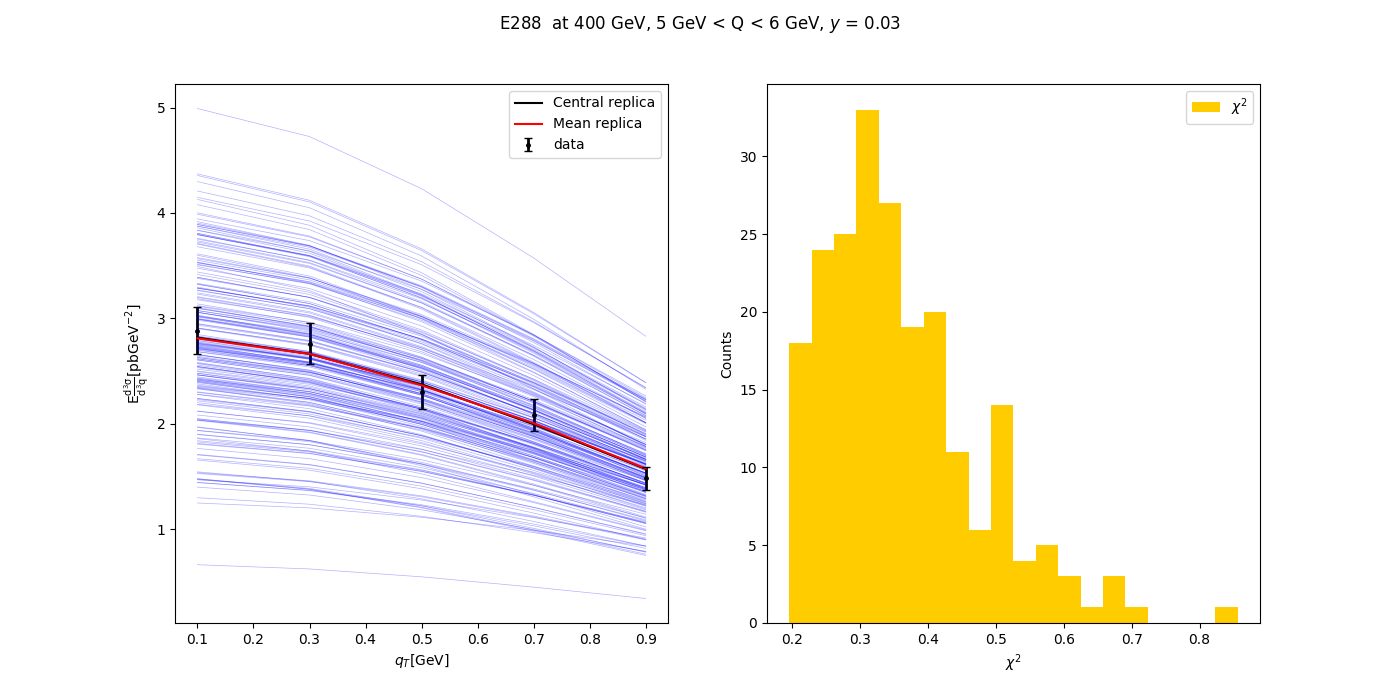
\includegraphics{pngplots/E288_400_Q_5_6.png}
\caption{E288\_400\_Q\_5\_6 data-theory comparison}
\end{figure}

\begin{figure}
\centering
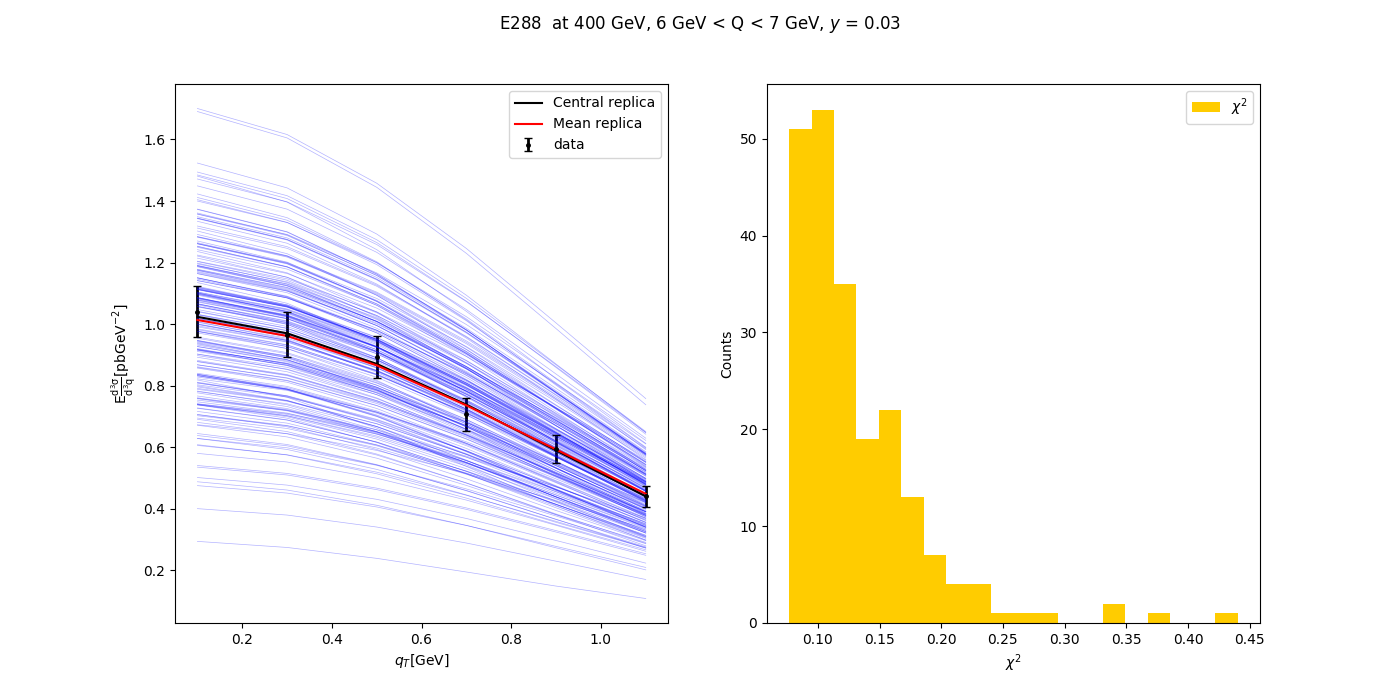
\includegraphics{pngplots/E288_400_Q_6_7.png}
\caption{E288\_400\_Q\_6\_7 data-theory comparison}
\end{figure}

\begin{figure}
\centering
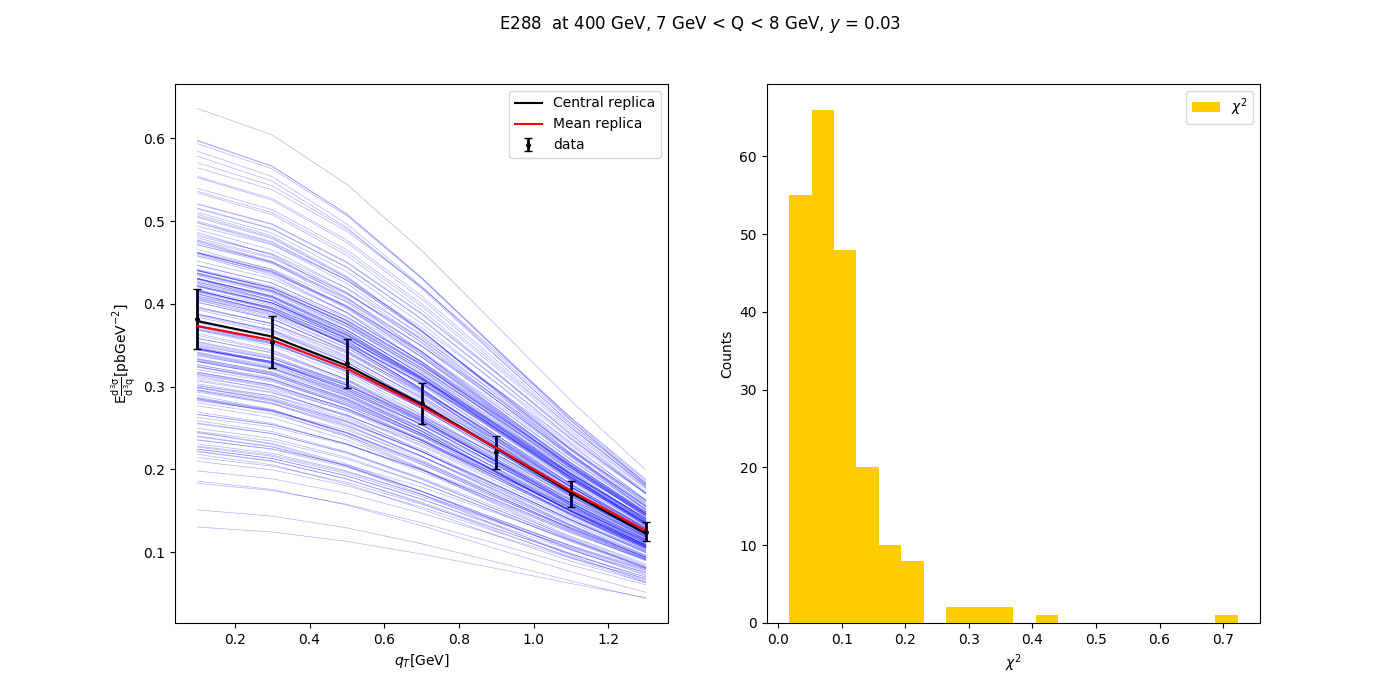
\includegraphics{pngplots/E288_400_Q_7_8.png}
\caption{E288\_400\_Q\_7\_8 data-theory comparison}
\end{figure}

\begin{figure}
\centering
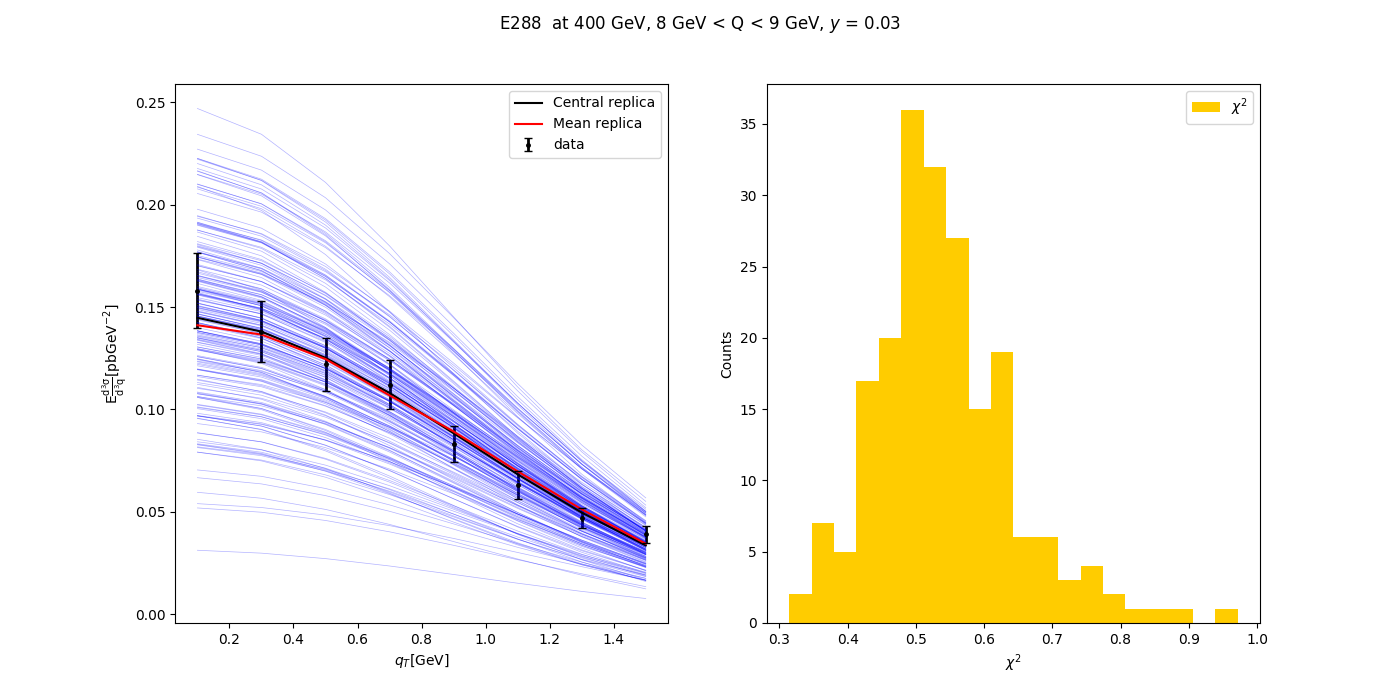
\includegraphics{pngplots/E288_400_Q_8_9.png}
\caption{E288\_400\_Q\_8\_9 data-theory comparison}
\end{figure}

\begin{figure}
\centering
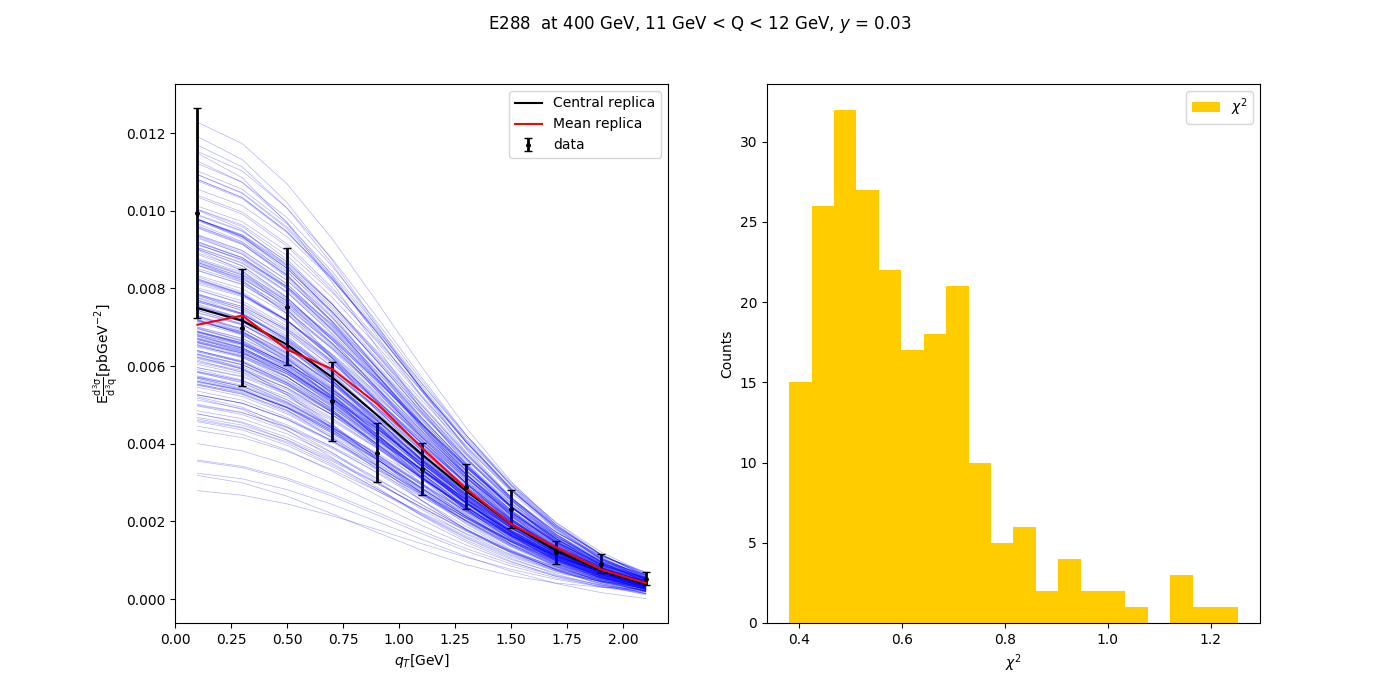
\includegraphics{pngplots/E288_400_Q_11_12.png}
\caption{E288\_400\_Q\_11\_12 data-theory comparison}
\end{figure}

\begin{figure}
\centering
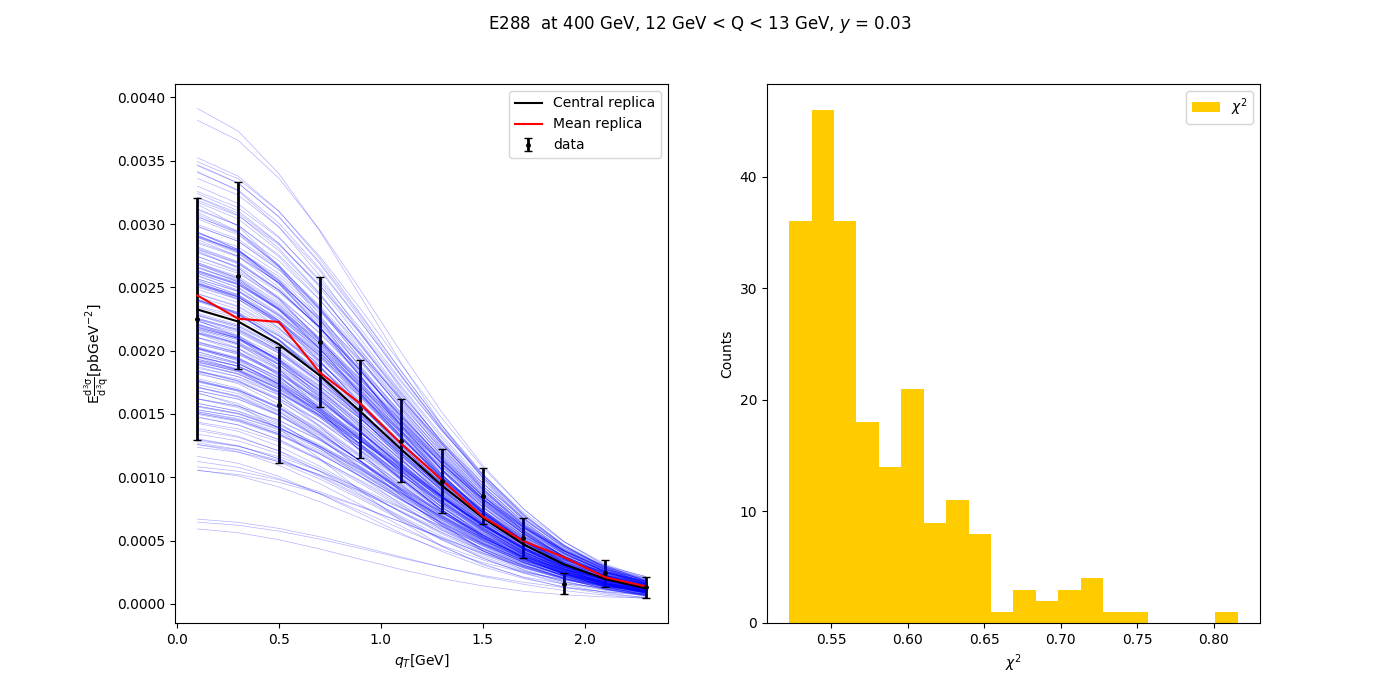
\includegraphics{pngplots/E288_400_Q_12_13.png}
\caption{E288\_400\_Q\_12\_13 data-theory comparison}
\end{figure}

\begin{figure}
\centering
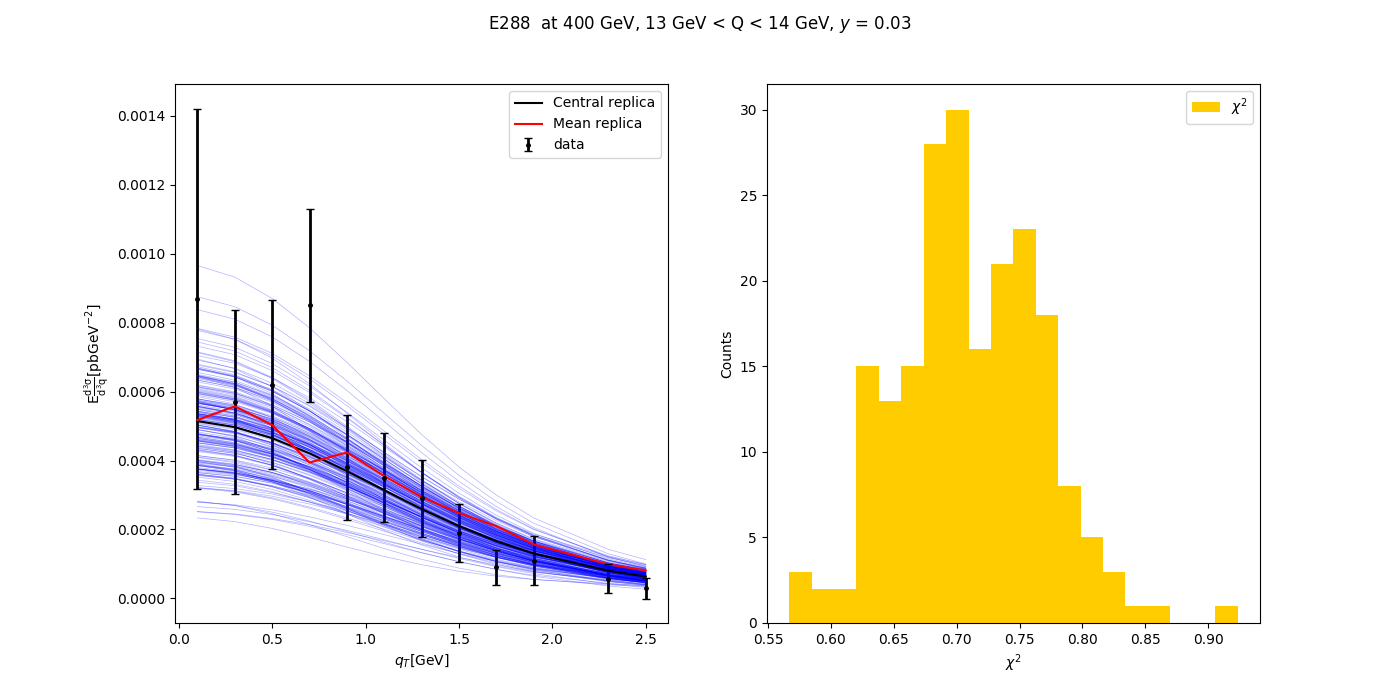
\includegraphics{pngplots/E288_400_Q_13_14.png}
\caption{E288\_400\_Q\_13\_14 data-theory comparison}
\end{figure}

\begin{figure}
\centering
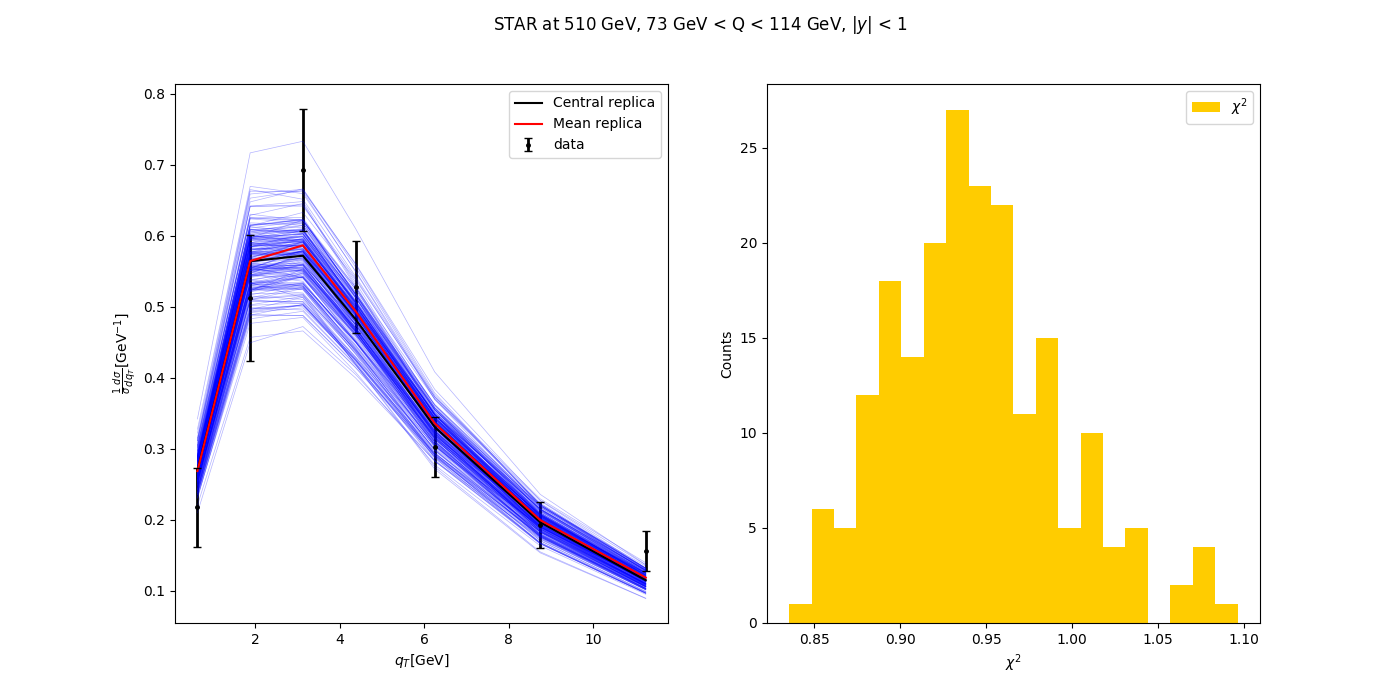
\includegraphics{pngplots/STAR_510.png}
\caption{STAR\_510 data-theory comparison}
\end{figure}

\begin{figure}
\centering
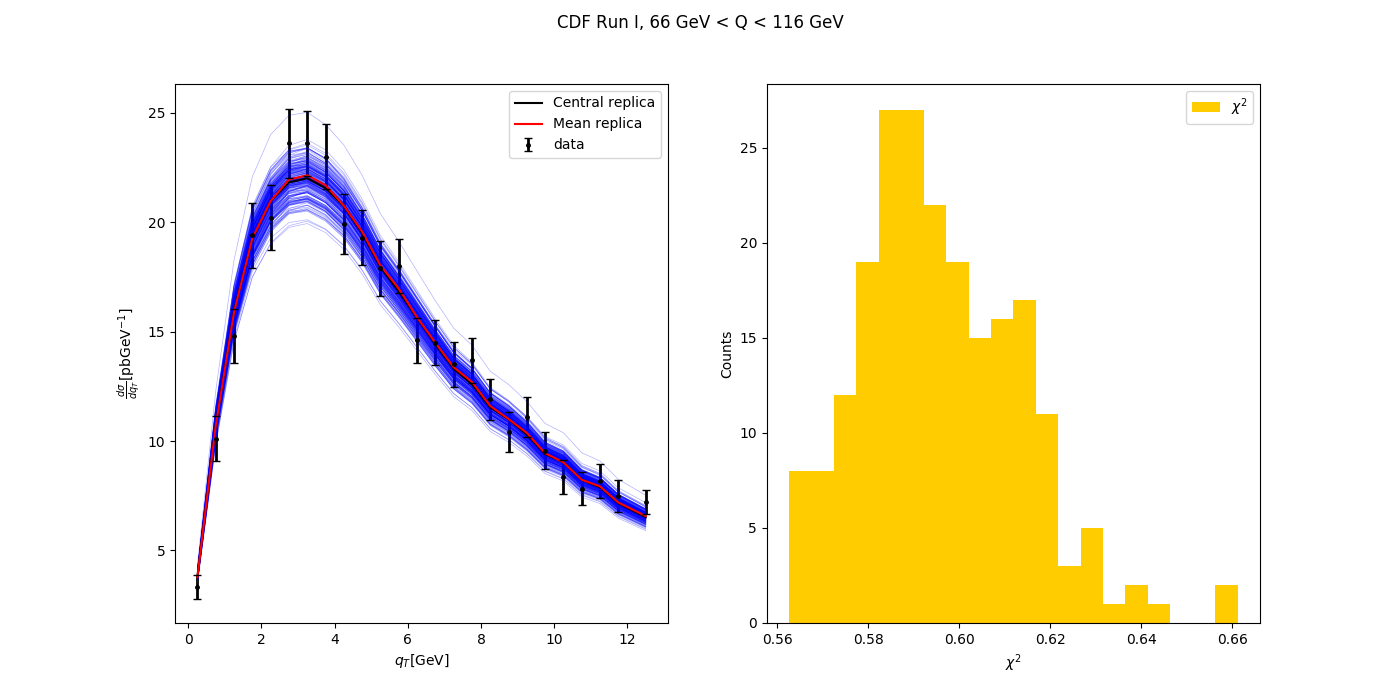
\includegraphics{pngplots/CDF_RunI.png}
\caption{CDF\_RunI data-theory comparison}
\end{figure}

\begin{figure}
\centering
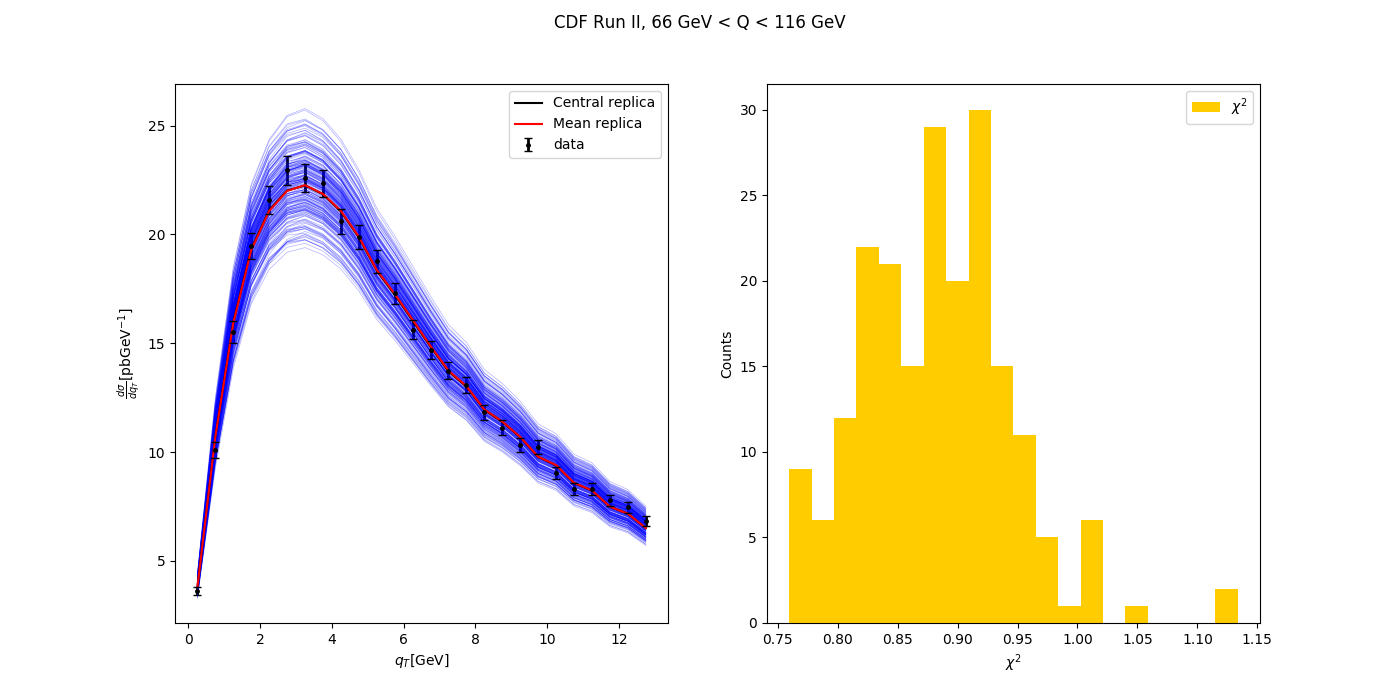
\includegraphics{pngplots/CDF_RunII.png}
\caption{CDF\_RunII data-theory comparison}
\end{figure}

\begin{figure}
\centering
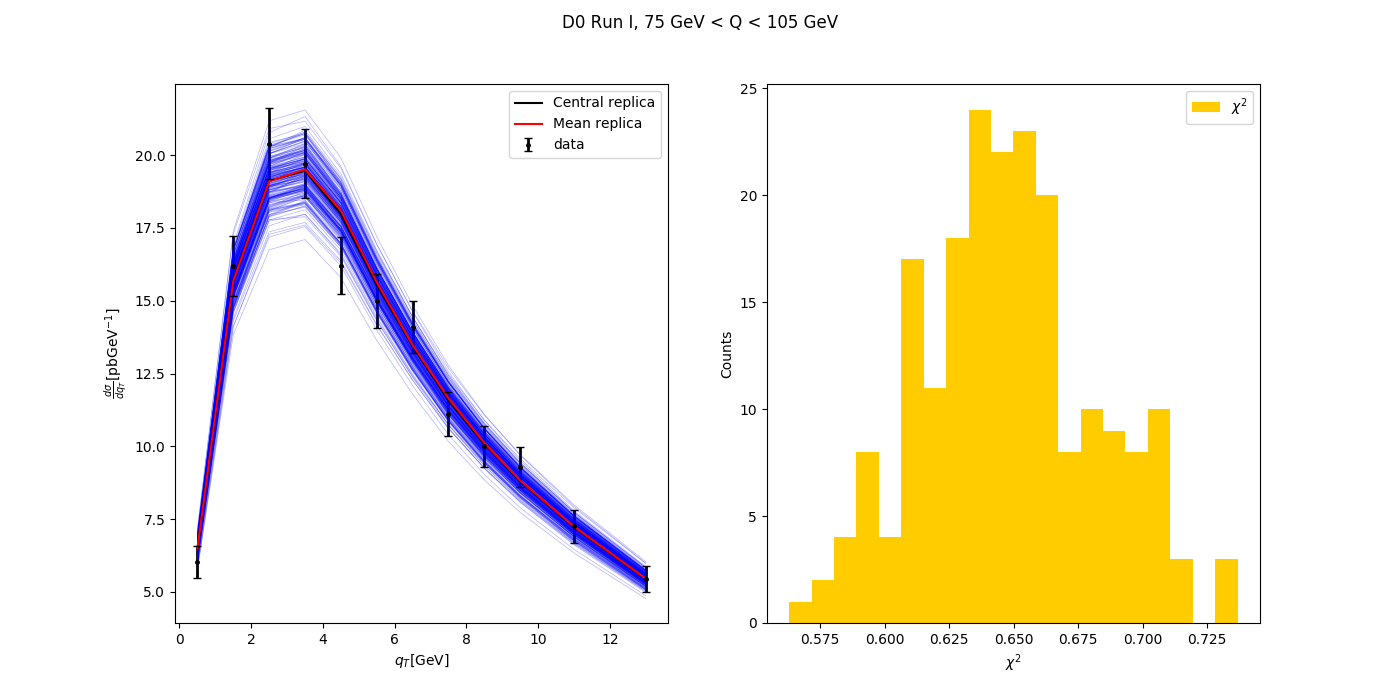
\includegraphics{pngplots/D0_RunI.png}
\caption{D0\_RunI data-theory comparison}
\end{figure}

\begin{figure}
\centering
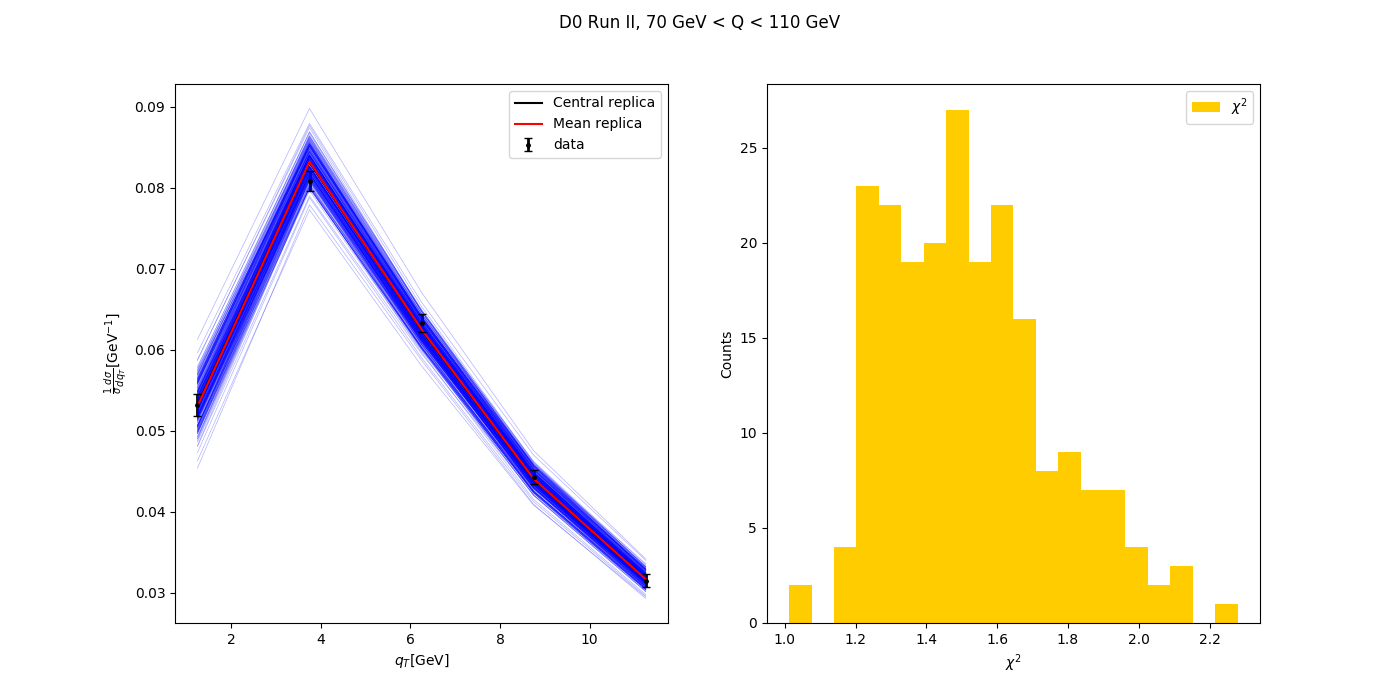
\includegraphics{pngplots/D0_RunII.png}
\caption{D0\_RunII data-theory comparison}
\end{figure}

\begin{figure}
\centering
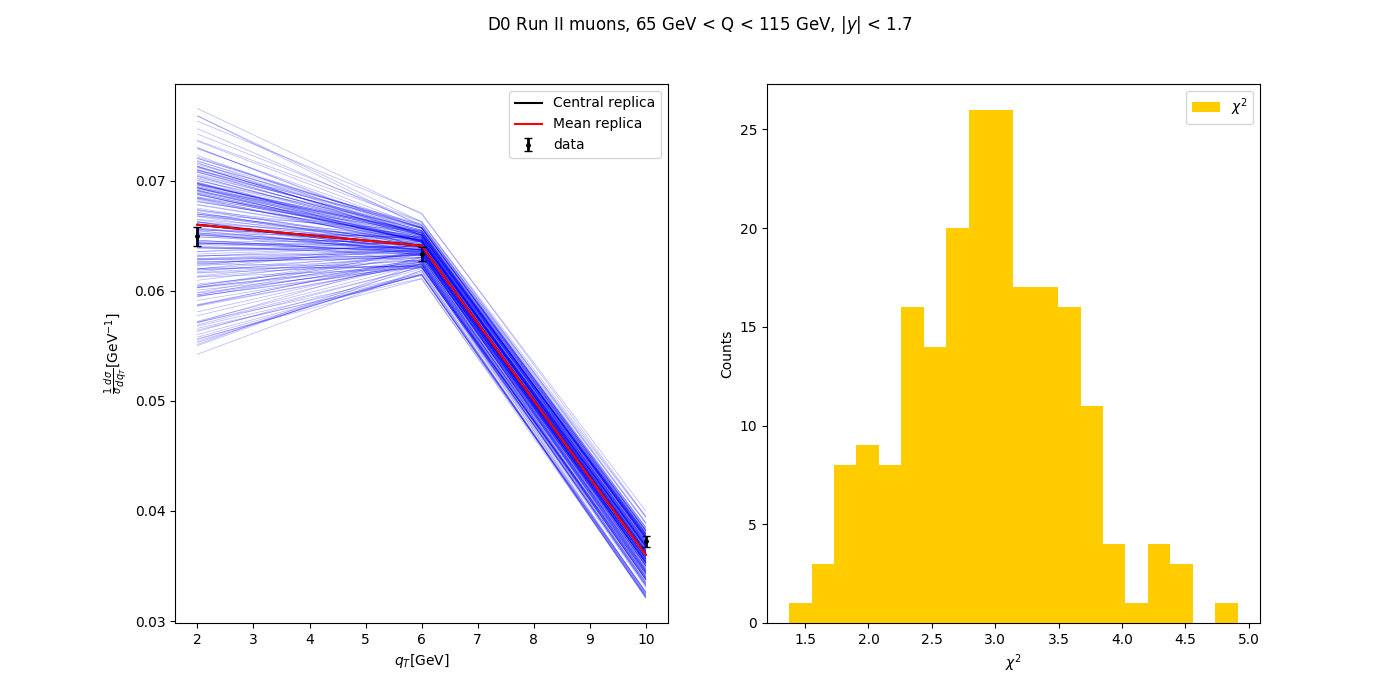
\includegraphics{pngplots/D0_RunIImu.png}
\caption{D0\_RunIImu data-theory comparison}
\end{figure}

\begin{figure}
\centering
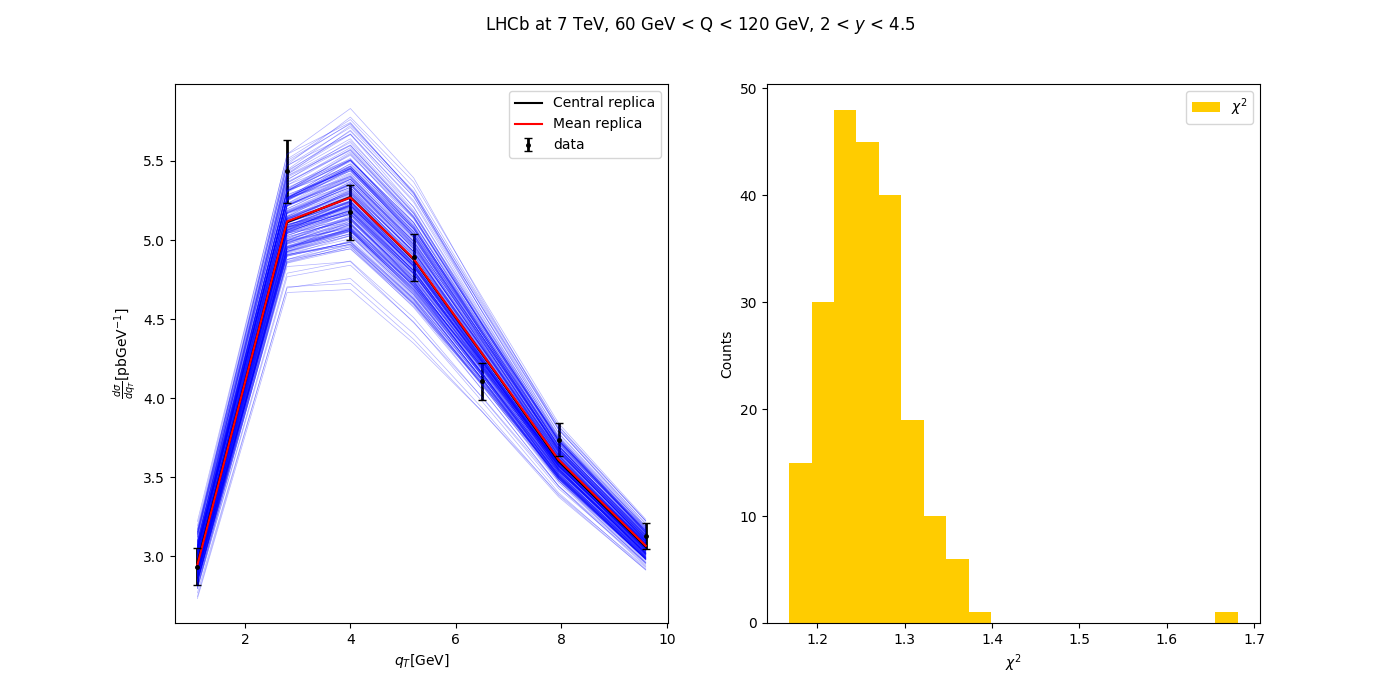
\includegraphics{pngplots/LHCb_7TeV.png}
\caption{LHCb\_7TeV data-theory comparison}
\end{figure}

\begin{figure}
\centering
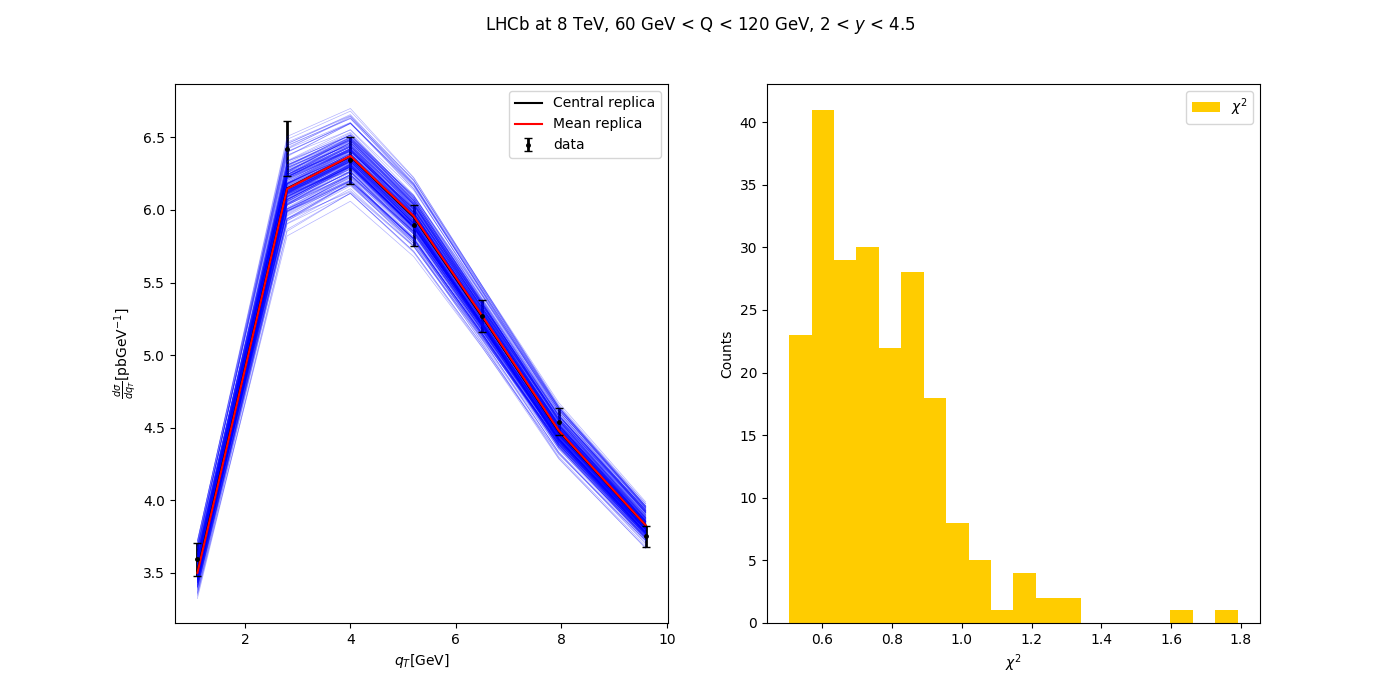
\includegraphics{pngplots/LHCb_8TeV.png}
\caption{LHCb\_8TeV data-theory comparison}
\end{figure}

\begin{figure}
\centering
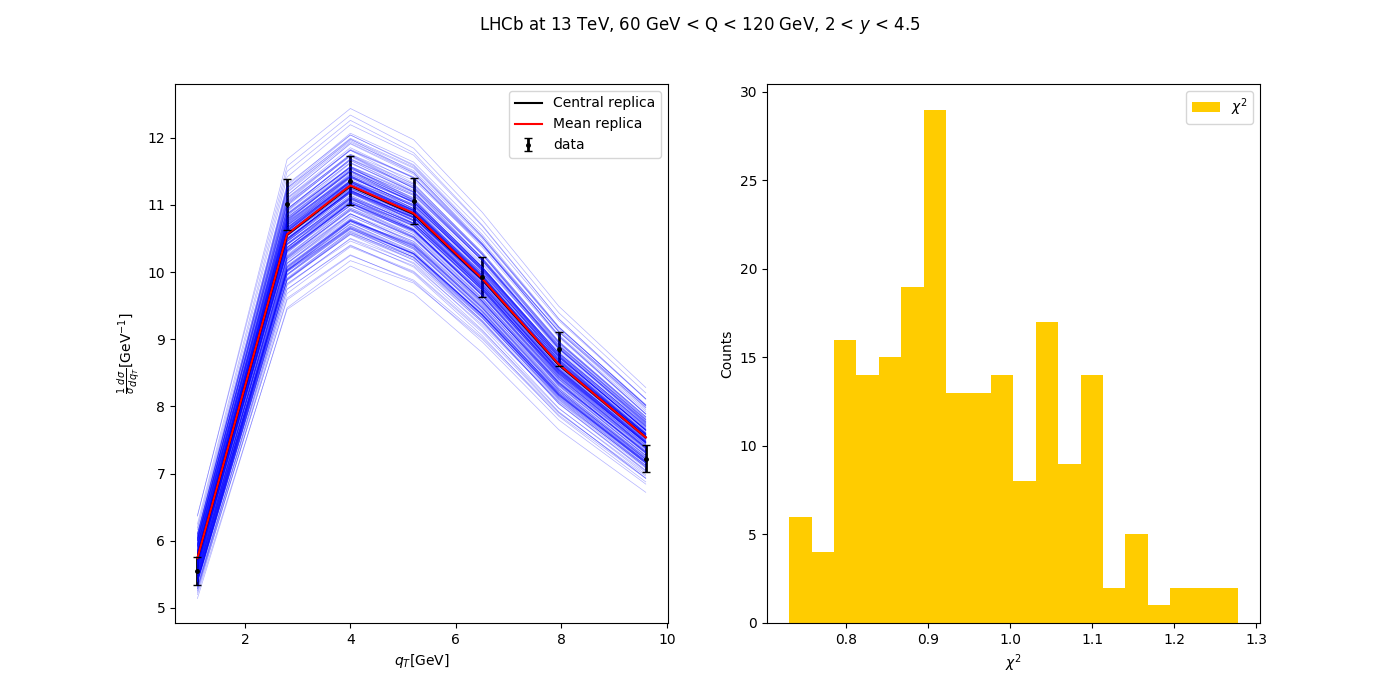
\includegraphics{pngplots/LHCb_13TeV.png}
\caption{LHCb\_13TeV data-theory comparison}
\end{figure}

\begin{figure}
\centering
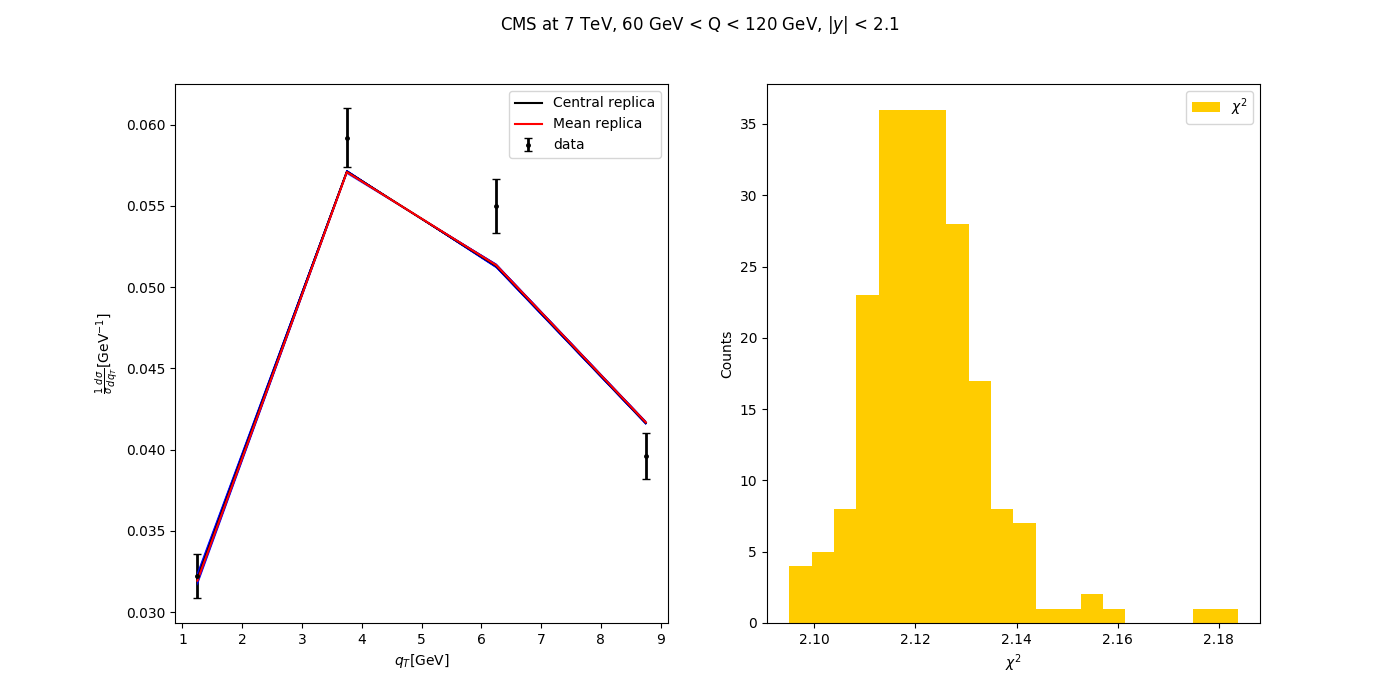
\includegraphics{pngplots/CMS_7TeV.png}
\caption{CMS\_7TeV data-theory comparison}
\end{figure}

\begin{figure}
\centering
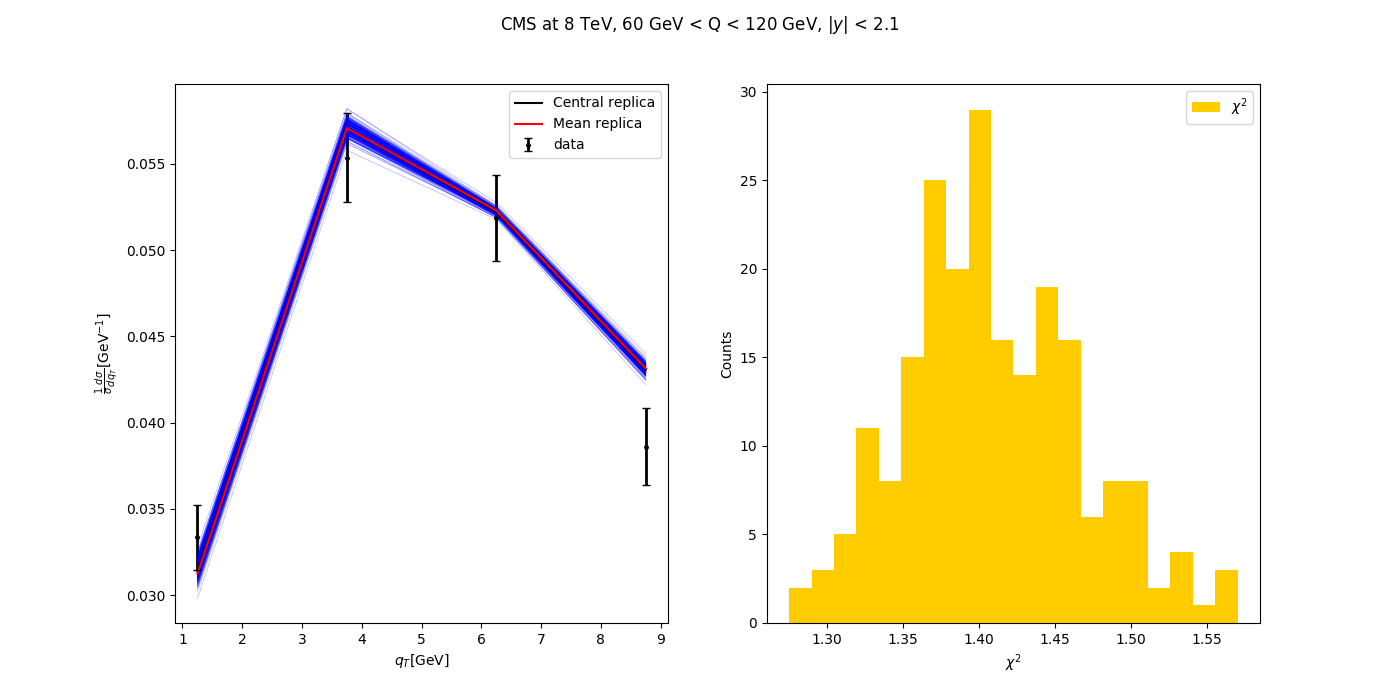
\includegraphics{pngplots/CMS_8TeV.png}
\caption{CMS\_8TeV data-theory comparison}
\end{figure}

\begin{figure}
\centering
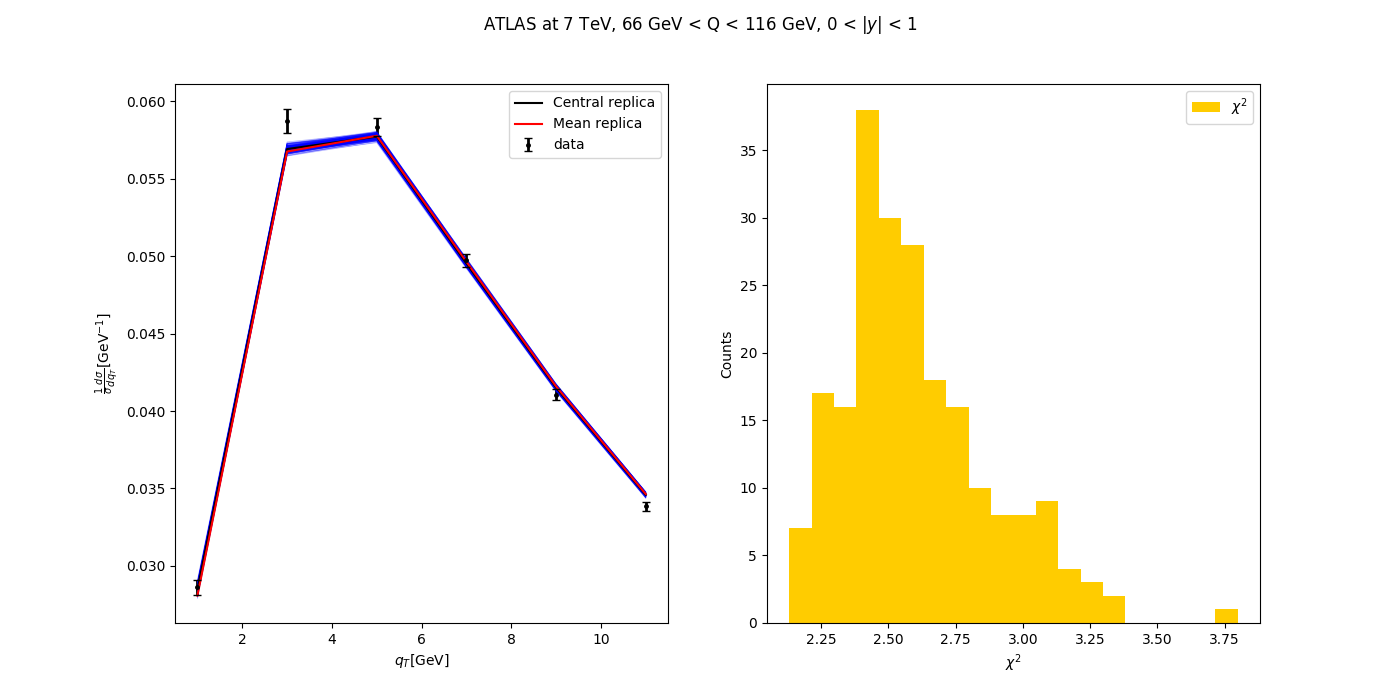
\includegraphics{pngplots/ATLAS_7TeV_y_0_1.png}
\caption{ATLAS\_7TeV\_y\_0\_1 data-theory comparison}
\end{figure}

\begin{figure}
\centering
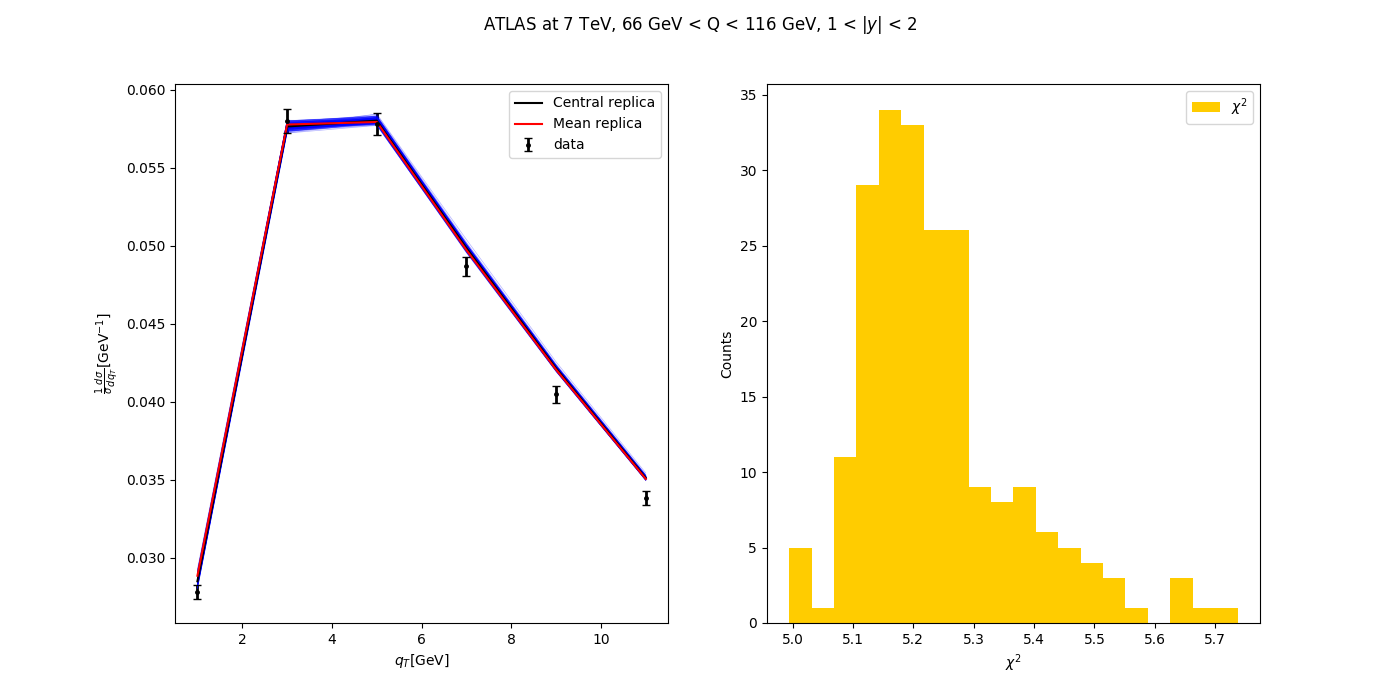
\includegraphics{pngplots/ATLAS_7TeV_y_1_2.png}
\caption{ATLAS\_7TeV\_y\_1\_2 data-theory comparison}
\end{figure}

\begin{figure}
\centering
\includegraphics{pngplots/ATLAS_7TeV_y_2_2.4.png}
\caption{ATLAS\_7TeV\_y\_2\_2.4 data-theory comparison}
\end{figure}

\begin{figure}
\centering
\includegraphics{pngplots/ATLAS_8TeV_y_0_0.4.png}
\caption{ATLAS\_8TeV\_y\_0\_0.4 data-theory comparison}
\end{figure}

\begin{figure}
\centering
\includegraphics{pngplots/ATLAS_8TeV_y_0.4_0.8.png}
\caption{ATLAS\_8TeV\_y\_0.4\_0.8 data-theory comparison}
\end{figure}

\begin{figure}
\centering
\includegraphics{pngplots/ATLAS_8TeV_y_0.8_1.2.png}
\caption{ATLAS\_8TeV\_y\_0.8\_1.2 data-theory comparison}
\end{figure}

\begin{figure}
\centering
\includegraphics{pngplots/ATLAS_8TeV_y_1.2_1.6.png}
\caption{ATLAS\_8TeV\_y\_1.2\_1.6 data-theory comparison}
\end{figure}

\begin{figure}
\centering
\includegraphics{pngplots/ATLAS_8TeV_y_1.6_2.png}
\caption{ATLAS\_8TeV\_y\_1.6\_2 data-theory comparison}
\end{figure}

\begin{figure}
\centering
\includegraphics{pngplots/ATLAS_8TeV_y_2_2.4.png}
\caption{ATLAS\_8TeV\_y\_2\_2.4 data-theory comparison}
\end{figure}

\begin{figure}
\centering
\includegraphics{pngplots/ATLAS_8TeV_Q_46_66.png}
\caption{ATLAS\_8TeV\_Q\_46\_66 data-theory comparison}
\end{figure}

\begin{figure}
\centering
\includegraphics{pngplots/ATLAS_8TeV_Q_116_150.png}
\caption{ATLAS\_8TeV\_Q\_116\_150 data-theory comparison}
\end{figure}

\end{document}
